%\documentclass[10pt, twocolumn]{article}
%\documentclass[11pt]{article}
%\documentclass[twocolumn,showpacs,preprintnumbers,amsmath,amssymb,prl, superscriptaddress]{revtex4}
\documentclass[twocolumn, preprintnumbers,amsmath,amssymb,prd, superscriptaddress]{revtex4}
% \documentclass[preprintnumbers,amsmath,amssymb,prd,superscriptaddress]{revtex4}
%\documentclass[10pt, preprint,showpacs,preprintnumbers,amsmath,amssymb, superscriptaddress]{revtex4}
%\documentclass[11pt, prd,preprintnumbers,amsmath,amssymb, superscriptaddress]{revtex4}
%\documentclass[11pt, prd,preprintnumbers, amsmath,amssymb, superscriptaddress, nofootinbib, hyperref]{revtex4}

\usepackage{latexsym}
\usepackage{amssymb}
\usepackage{epsfig,amsmath,graphics}
\usepackage{epstopdf}
\usepackage{verbatim}
\usepackage{wasysym}
\usepackage{hyperref}
\usepackage{feynmp-auto} % feynman diagrams
%\usepackage{subfig}
\usepackage[utf8]{inputenc}
\usepackage{xpatch}
\usepackage{xcolor}
\usepackage{mathtools}
\hypersetup{
    colorlinks,
    linkcolor={red!80!black},
    citecolor={green!60!black},
    urlcolor={blue!60!black}
}
\usepackage{appendix}

\newcommand{\Ez}{\mathcal{E}_0}
\newcommand{\Eboom}{\mathcal{E}_\text{boom}}
\newcommand{\OO}{\mathcal{O}}
\newcommand{\LL}{\mathcal{L}}
\newcommand{\HH}{\mathcal{H}}
\newcommand{\TeV}{\text{TeV}}
\newcommand{\GeV}{\text{GeV}}
\newcommand{\MeV}{\text{MeV}}
\newcommand{\keV}{\text{keV}}
\newcommand{\rad}{\text{rad}}
\newcommand{\cm}{\text{cm}}
\newcommand{\angstrom}{\buildrel _{\circ} \over {\mathrm{A}}}
\newcommand{\pslash}{p\hspace{-0.070in}/\,}
\newcommand{\Mpl}{M_{\text{pl}}}
\newcommand{\ket}[1]{\ensuremath{\left|#1\right>}}
\newcommand{\bra}[1]{\ensuremath{\left<#1\right|}}
\newcommand{\braket}[2]{\ensuremath{\left<#1|#2\right>}}
%Large Parentheses
\def\r{\right)}
\def\l{\left(}

\begin{document}

%\preprint{APS/123-QED}


\title{White Dwarfs as Dark Matter Detectors}

\author{Peter W. Graham}
\affiliation{Stanford Institute for Theoretical Physics, Department of Physics,
Stanford University, Stanford, CA, 94305}

\author{Ryan Janish}
\affiliation{Berkeley Center for Theoretical Physics, Department of Physics,
University of California, Berkeley, CA 94720, USA}

\author{Vijay Narayan}
\affiliation{Berkeley Center for Theoretical Physics, Department of Physics,
University of California, Berkeley, CA 94720, USA}

\author{Surjeet Rajendran}
\affiliation{Berkeley Center for Theoretical Physics, Department of Physics,
University of California, Berkeley, CA 94720, USA}

\author{Paul Riggins}
\affiliation{Berkeley Center for Theoretical Physics, Department of Physics,
University of California, Berkeley, CA 94720, USA}

\begin{abstract}

If dark matter (DM) is capable of sufficiently heating a local region in a white dwarf, it will trigger runaway fusion and ignite a type 1a supernova.
This was originally proposed in \cite{Graham:2015apa} and used to constrain primordial black holes which transit and heat a white dwarf via dynamical friction.
% In this paper, we extend the reach of white dwarf DM detectors to candidates with non-gravitational interactions that cause heating through the release of standard model particles.
In this paper, we extend the analysis of white dwarf DM detection to candidates with non-gravitational interactions that heat through the production of standard model particles.
We consider a general class of models in which DM-DM collisions, DM decays, or DM transits including a SM scattering interaction produce particles that subsequently deposit energy inside the star.
The existence of long-lived white dwarfs and the observed supernova rate provide robust for constraints for such models.
As a concrete example, we rule out supersymmetric Q-ball DM in a vast region of parameter space fundamentally inaccessible to terrestrial detection.
It is also intriguing that the DM-induced SN discussed in this work provide an alternative mechanism of triggering supernovae from sub-Chandrasekhar Mass progenitors.


\end{abstract}
\maketitle
\onecolumngrid
\tableofcontents
\clearpage
\twocolumngrid

\section{Introduction}
\label{sec:Introduction}

Identifying the nature of dark matter (DM) remains one of the clearest paths beyond the Standard Model (SM) and it is thus fruitful to study the observable signatures of any yet-allowed candidate.
Many terrestrial direct detection experiments are designed to search for DM, e.g.~\cite{Akerib:2016vxi, Agnese:2017njq}, yet these lose sensitivity to heavier DM due to its diminished number density.
Even for a strongly-interacting candidate, if the DM mass is above $\sim 10^{22} ~\GeV$ a large detector of size $\sim (100 ~\text{m})^2$ will register fewer than one event per year.
While these masses are large compared to those of fundamental particles, it is reasonable to suppose that DM may exist as composite states just as the SM produces complex structures with mass much larger than fundamental scales (e.g. you, dear reader).
Currently there is a wide range of unexplored parameter space for DM candidates less than $\sim 10^{48} ~\GeV$, above which the DM will have observable gravitational microlensing effects \cite{Griest:2013aaa}.
For such ultra-heavy DM, indirect signatures in astrophysical systems are a natural way forward.
One possibility proposed by \cite{Graham:2015apa} is that DM can trigger runaway fusion and ignite type 1a supernovae (SN) in sub-Chandrasekhar white dwarf (WD) stars.
This process is even more interesting in light of recent observations which find that an $\OO(1)$ fraction of type 1a SN occur via sub-Chandrasekhar progenitors~\cite{Scalzo:2014sap, Scalzo:2014wxa}.
While astrophysical mechanisms for these events have been proposed \cite{Woosley1994,Fink:2007fv}, the situation is yet unclear and it is an exciting possibility that these SN arise from DM interactions.

Runaway thermonuclear fusion requires both a heating event and the lack of significant cooling which might quench the process.
The WD medium is particularly suited to this as it is dominated by degeneracy pressure and undergoes minimal thermal expansion, which is the mechanism that regulates fusion in main sequence stars.
Thermal diffusion is the primary cooling process in a WD and it can be thwarted by heating a large enough region.
The properties of a localized heating necessary to trigger runaway fusion were computed in \cite{Woosley}.
Consequently, \cite{Graham:2015apa} realized that if DM is capable of sufficiently heating a WD in this manner, it will result in a SN with sub-Chandrasekhar Mass progenitor.
This was used to constrain primordial black holes which transit a WD and cause heating by dynamical friction, although the authors of \cite{Graham:2015apa} identify several other heating mechanisms which may be similarly constrained.

In this paper, we examine DM candidates with non-gravitational interactions that cause heating through the production of SM particles.
An essential ingredient in this analysis is understanding the length scales over which SM particles deposit energy in a WD medium.
We find that most high energy particles thermalize efficiently with ions in the WD, nearly independent of species or initial energy.
Particle production is thus an effective means of inducing SN.
Constraints on these DM candidates come from either observing specific, long-lived WDs or by comparing the measured rate of type 1a SN with that expected due to DM.
It is important to note that these constraints are complementary to direct searches---it is more massive DM that is likely to trigger SN, but also more massive DM that has low terrestrial flux.
The WD detector excels in this regime due to its large surface area $\sim (10^4 ~\text{km})^2$, long lifetime $\sim \text{Gyr}$, and galactic abundance.
We demonstrate these constraints for generic classes of DM models that produce SM particles via DM-DM collisions, DM decays, or DM transits including a SM scattering interaction.
As a concrete example we consider ultra-heavy Q-ball DM as found in supersymmetric extensions of the SM, which we rule out in a vast region of parameter space.

The rest of the paper is organized as follows.
We begin in Section~\ref{sec:Review} by reviewing the mechanism of runaway fusion in a WD.
In Section~\ref{sec:SMHeating} we study the non-gravitational heating of a WD due to the production of high-energy SM particles.
Detailed calculations of the stopping of such particles are provided in Appendix \ref{sec:wdpdg}.
In Section~\ref{sec:DMexplode} we parameterize the explosiveness and rate of events for generic classes of DM-WD encounters, and in Section~\ref{sec:Constraints} we derive schematic constraints on such models using WD observables.
Finally we specialize to the case of Q-balls in Section~\ref{sec:QBalls}, and conclude in Section~\ref{sec:Discussion}.

\section{White Dwarf Runaway Fusion}
\label{sec:Review}

We first review the conditions for which a local energy deposition in a WD results in runaway fusion.
Any energy deposit will eventually heat ions within some localized region---parameterize this region by its linear size $L_0$, total kinetic energy $\Ez$ and typical temperature $T_0$.
These scales evolve in time, but it will be useful to describe a given heating event by their initial values.

The fate of a heated region is either a nonviolent diffusion of the excess energy across the star, or a runaway fusion chain-reaction that destroys the star.
The precise outcome depends on $L_0$, $\Ez$ and $T_0$.
There is a critical temperature $T_f$, set by the energy required for ions to overcome their mutual Coulomb barrier, above which fusion occurs.
For carbon burning, $T_f \sim \MeV$ \cite{Gasques:2005ar}.
Any heated region $T_0 > T_f$ will initially support fusion, although this is not sufficient for runaway as cooling processes may rapidly lower the temperature below $T_f$.
This cooling will not occur if the corresponding timescale is larger than the timescale at which fusion releases energy.
Cooling in a WD is dominated by thermal diffusion, and the diffusion time increases as the size of the heated region.
However, the timescale for heating due to fusion is independent of region size.
Thus, for a region at temperature $\geq T_f$, there is a critical size above which the heated region does not cool but instead initiates runaway.
For a region at the critical fusion temperature $T_f$, we call this critical size the \emph{trigger size} $\lambda_T$.
The value of $\lambda_T$ is highly dependent on density, and in a WD is set by the thermal diffusivity of either photons or degenerate electrons.
This critical length scale has been computed numerically in \cite{Woosley} for a narrow range of WD densities and analytically scaled for other WD masses in \cite{Graham:2015apa}.
As in \cite{Graham:2015apa}, we will restrict our attention to carbon-oxygen WDs in the upper mass range $\sim 0.85 - 1.4 ~M_{\odot}$ (these will yield the most stringent constraints on DM).
This corresponds to a central number density of ions $n_\text{ion} \sim 10^{30} - 10^{32} ~\cm^{-3}$ and a trigger size of $\lambda_T \sim 10^{-3} - 10^{-5} ~\text{cm}$.

If a heated region is smaller than the trigger size, its thermal evolution is initially dominated by diffusion.
However, this will still result in runaway fusion if the temperature is of order $T_f$ by the time the region diffuses out to the trigger size.
For our purposes it is more natural to phrase this in terms of the total energy $\Ez$ deposited during a heating event.
Of course, the relation between energy $\Ez$ and temperature $T_0$ depends on the rate at which WD constituents---ions, electrons, and photons---thermalize with each other within the region size $L_0$.
In Section \ref{sec:SMHeating} we explicitly calculate the length scales over which a hot bath of ions thermalizes electrons and photons, focusing our attention on ions because they are what ultimately must be heated in order for fusion to take place.
Here we simply state the results: if ions are heated to temperatures $T_0 \sim 1 - 10 ~\MeV$, which we will see is typical for a wide variety of heating processes, then electrons and photons are also heated to $T_0$ within the trigger size.
Therefore, any heating event which results in runaway necessarily has ions, electrons, and photons in thermal equilibrium once a region of size $\lambda_T$ or greater is at the critical temperature $T_f$.
The excess energy in a volume $V$ required to heat all these species to $T_f$ is given by a sum of their heat capacities
\begin{equation}
\label{eq:heatcapacity}
  \frac{\Ez}{V} \gtrsim \int_0^{T_f} dT ~\left(\frac32 n_\text{ion} + \frac{\pi^{4/3}}{3^{1/3}}\, n_e^{2/3} T + \frac{4 \pi^2}{15} T^3 \right),
\end{equation}
where $n_e$ is the number density of electrons.
Note that we use the heat capacity of a degenerate gas of electrons, since the Fermi energy $E_F \gtrsim \MeV$ for the densities we consider.
The minimum energy deposit necessary to trigger runaway fusion is simply
\begin{align}
\label{eq:Eboom}
\Eboom &\sim \frac{4 \pi}{3} \lambda_T^3 (n_\text{ion} T_f + n_e^{2/3} T_f^2 + T_f^4) \\
         &\approx 10^{15} - 10^{23} ~\GeV \nonumber.
\end{align}
$\Eboom$ varies with $\lambda_T$ over the range of WD densities and is plotted in Figure \ref{fig:Eboom}.
Thus for a heating event characterized by its $L_0$, $\Ez$, and any $T_0 \gtrsim T_f$, there is a \emph{boom condition}:
\begin{align}
    \label{eq:energy_boom_condition}
    \Ez \gtrsim
    \Eboom \cdot \text{max}\left\{1, \frac{L_0}{\lambda_T}\right\}^3.
\end{align}
Any $\Ez$ satisfying this condition is minimized for $L_0$ less than the trigger size, where it is also independent of the precise value of $L_0$.
For broader deposits, the necessary energy is parametrically larger than $\Eboom$ by a volume ratio $(L_0/\lambda_T)^3$.
As a result, understanding the $L_0$ for different kinds of heating events in a WD is critical to determining whether or not they are capable of destroying the star.
\begin{figure}
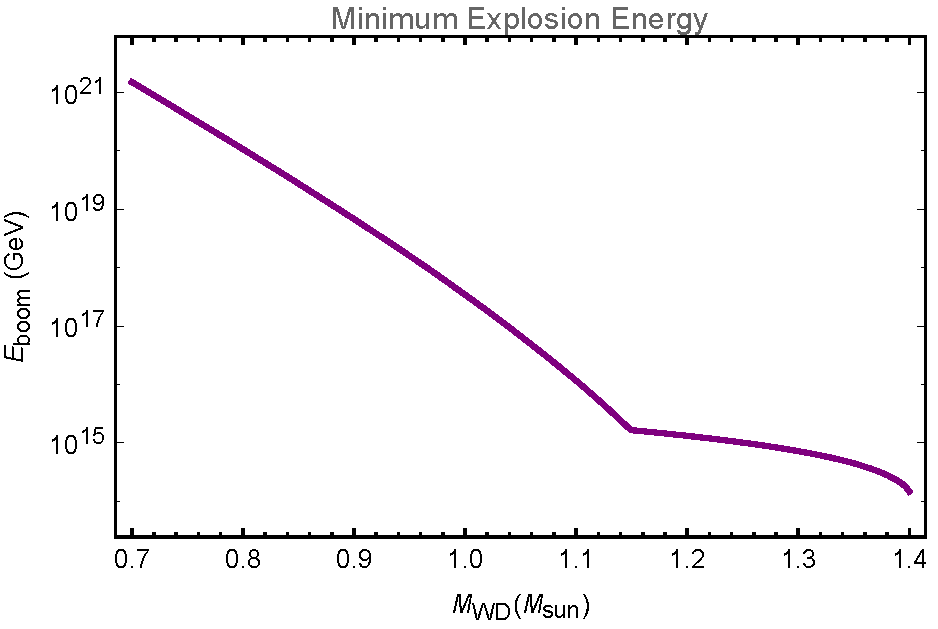
\includegraphics[scale=.45]{Eboom.pdf}
\caption{The minimum energy deposit \eqref{eq:Eboom} necessary to trigger runaway fusion, based on numerical results for $\lambda_T$ \cite{Woosley} and the WD mass-density relation \cite{cococubed}}.
\label{fig:Eboom}
\end{figure}

\section{Non-Gravitational Heating of White Dwarfs}
\label{sec:SMHeating}

We address now the possibility of DM heating the WD medium via the production of SM particles.
The critical quantity is the length scale over which such SM particles heat the medium---this scale determines their efficiency in triggering runaway fusion, as described by condition \eqref{eq:energy_boom_condition}.
Note that this is a question of purely SM physics.
The unknown physics of DM will serve only to set the initial properties of the SM particles.

One may have expected that efficient heating occurs only for a limited range of SM species and energies, thus restricting the set of DM candidates capable of producing SN.
However, we find that SM particles tend to efficiently heat the WD regardless of species or energy---the length scale of heating is typically less than or of order the trigger size $\lambda_T$, and is never parametrically larger.
This is accomplished primarily through hadronic showers initiated by collisions with carbon ions.
In some cases electromagnetic showers are important, however at high energies radiative processes are suppressed by density effects and all species are dominated by hadronic interactions.
These interactions rapidly stop high-energy particles due to the logarithmic nature of showers, converting them into a cloud of low-energy particles which efficiently heat the WD medium through elastic scatters.
In this light, the WD operates analogously to a particle detector, including hadronic and electromagnetic ``calorimeter'' components.
Runaway fusion provides the necessary amplification to convert a detected event into a recordable signal, in this case a violent SN.

In the remainder of this section we present the above heating process in more detail.
We summarize the dominant source of energy loss and the resulting ranges $\lambda$ for SM particles of incident energy $\epsilon$, approximated by
\begin{align}
    \lambda \sim \frac{\epsilon}{dE/dx}
\end{align}
where $dE/dx$ is the stopping power in the WD medium.
These are plotted in  Figures \ref{fig:SPhighEM}, \ref{fig:SPlowEM}, \ref{fig:SPhighHad}, and \ref{fig:SPlowHad}.
A detailed treatment of the stopping powers is reserved for Appendix \ref{sec:wdpdg}, while here we collect and discuss the results.
We will consider incident electrons, photons, light hadrons, and neutrinos, and since we are concerned with triggering runaway fusion we take $\epsilon \gg T_f \sim \text{MeV}$.
Note that an explosive heating event may consist of either producing a few highly energetic particles, or $N \gg 1$ low-energy particles.
These scenarios may have very different heating lengths, and we will distinguish between them when applicable.

\begin{figure}
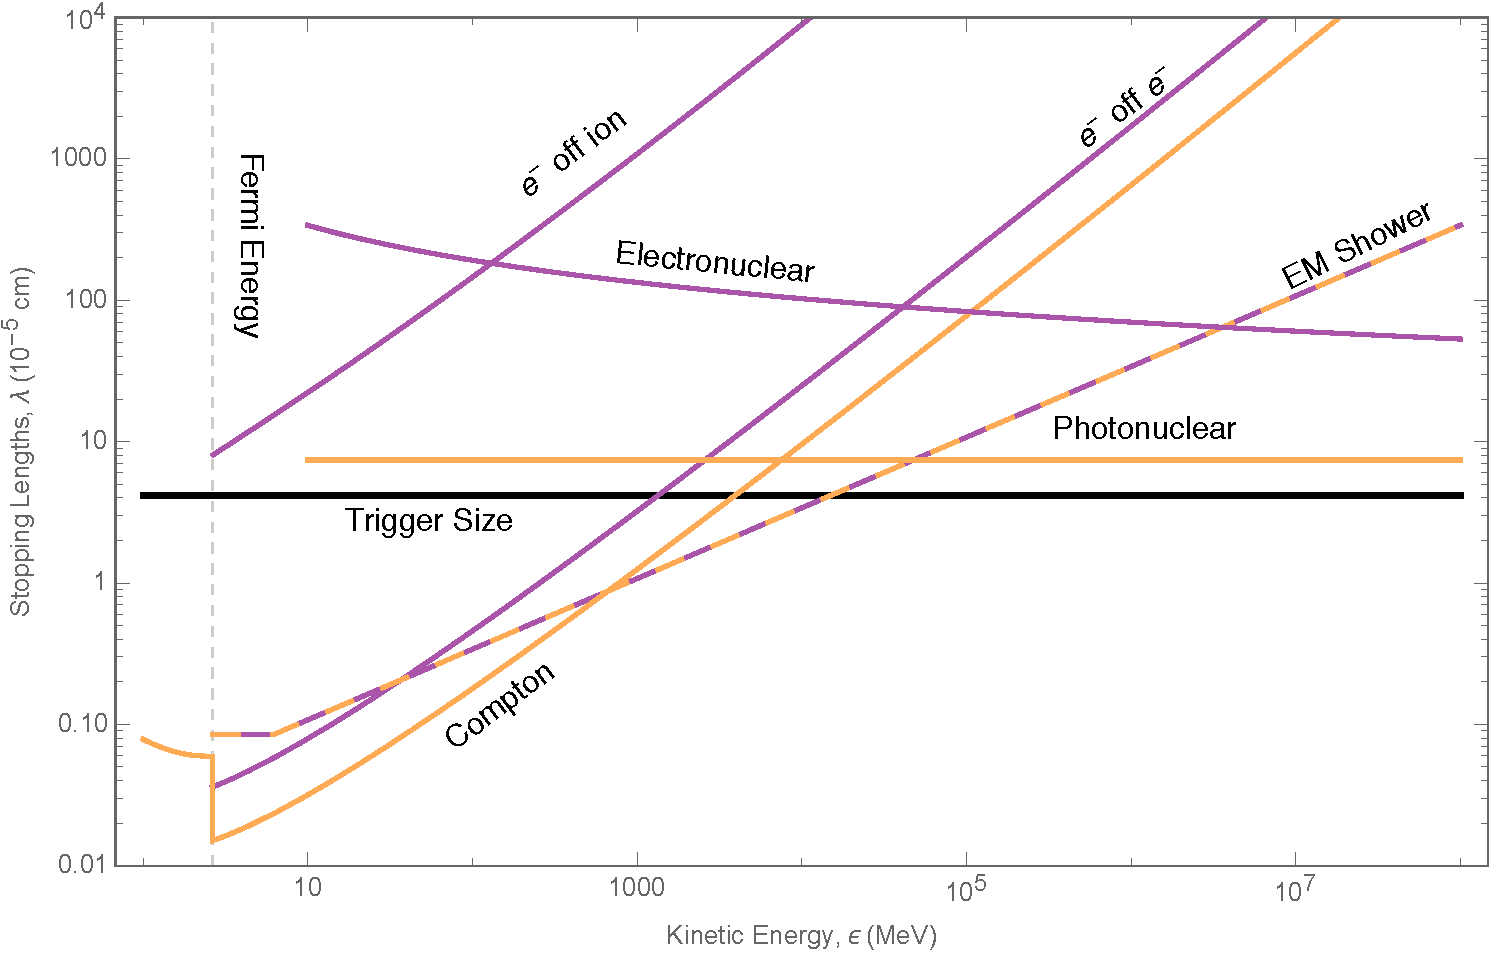
\includegraphics[scale=.3]{SPhighEM.pdf}
\caption{Stopping lengths for incident electrons and photons, plotted versus incident kinetic energy at high densities: $n_\text{ion}~\approx~10^{32}~\text{cm}^{-3}$, $M_\text{WD} \approx 1.37 M_{\astrosun}$. Orange lines are incident photons, purple lines are incident electrons.}
\label{fig:SPhighEM}
\end{figure}

\begin{figure}
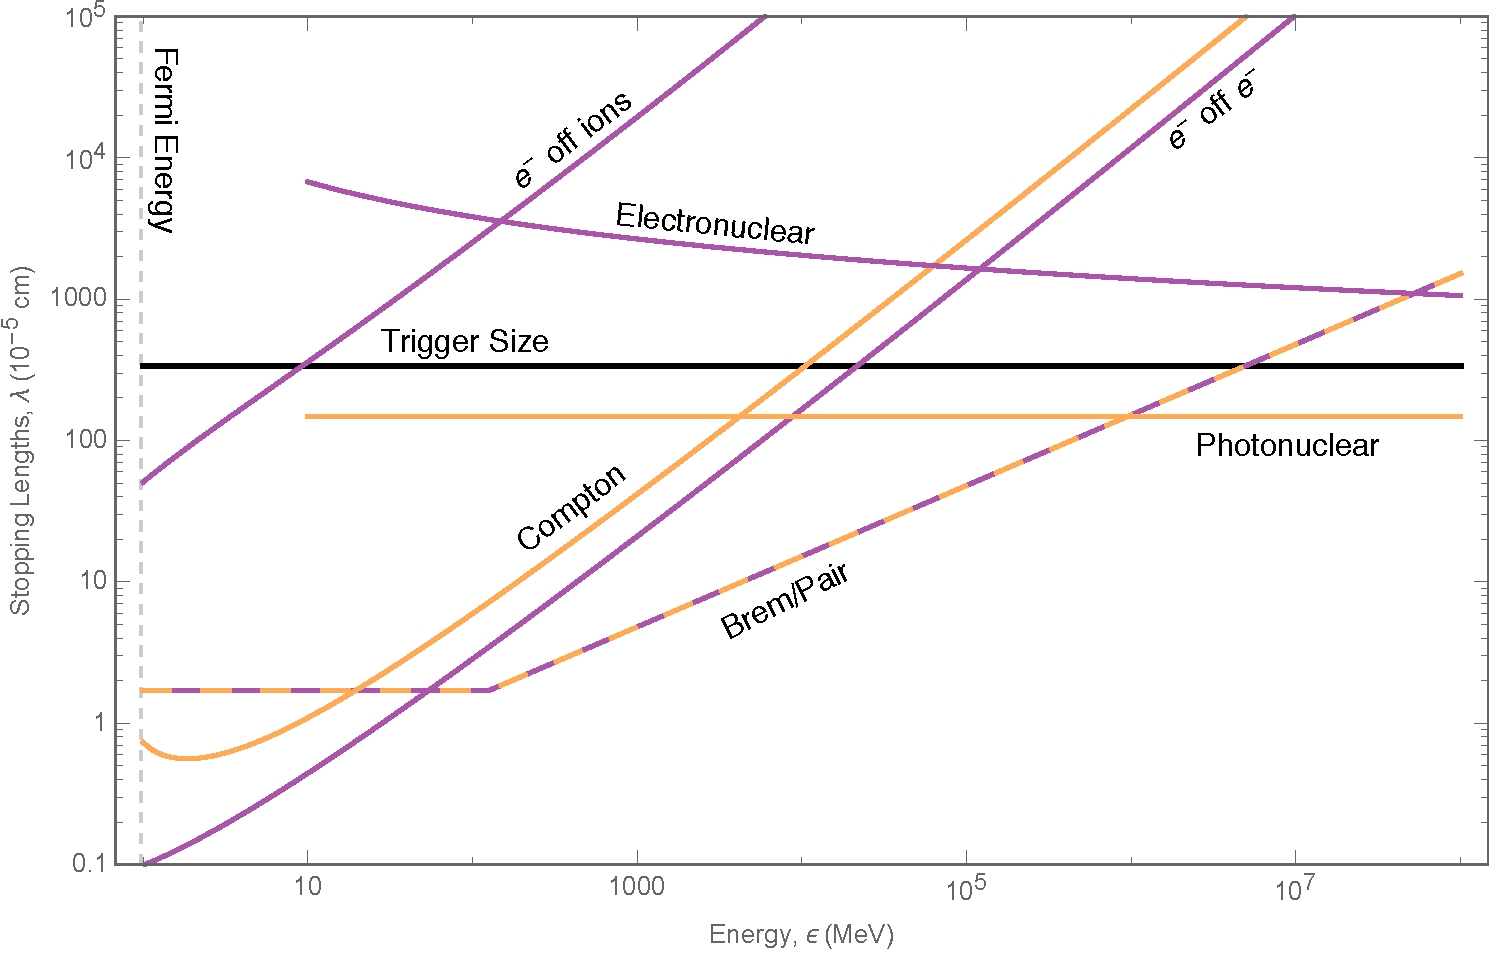
\includegraphics[scale=.3]{SPlowEM.pdf}
\caption{Stopping lengths for incident electrons and photons. plotted versus incident kinetic energy at low densities: $n_\text{ion}~\approx~10^{30}~\text{cm}^{-3}$, $M_\text{WD} \approx 0.85 M_{\astrosun}$. Orange lines are incident photons, purple lines are incident electrons.}
\label{fig:SPlowEM}
\end{figure}

\begin{figure}
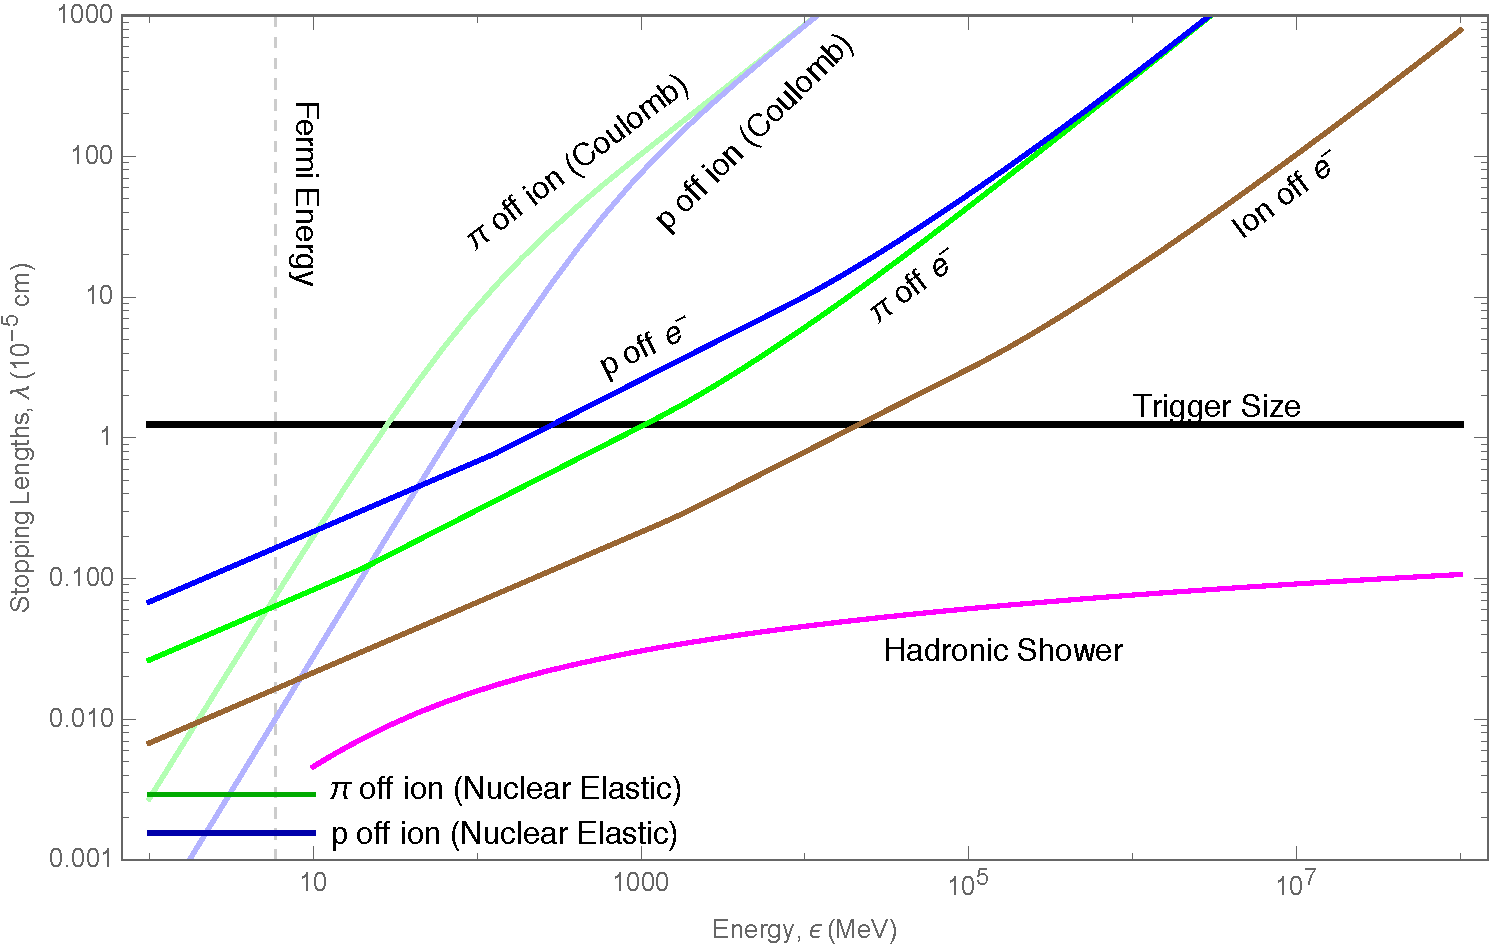
\includegraphics[scale=.3]{SPhighHad.pdf}
\caption{Stopping lengths for incident hadrons, plotted versus incident kinetic energy at high densities: $n_\text{ion}~\approx~10^{32}~\text{cm}^{-3}$, $M_\text{WD} \approx 1.37 M_{\astrosun}$. The magenta line is the hadronic shower length $X_\text{had}$.}
\label{fig:SPhighHad}
\end{figure}

\begin{figure}
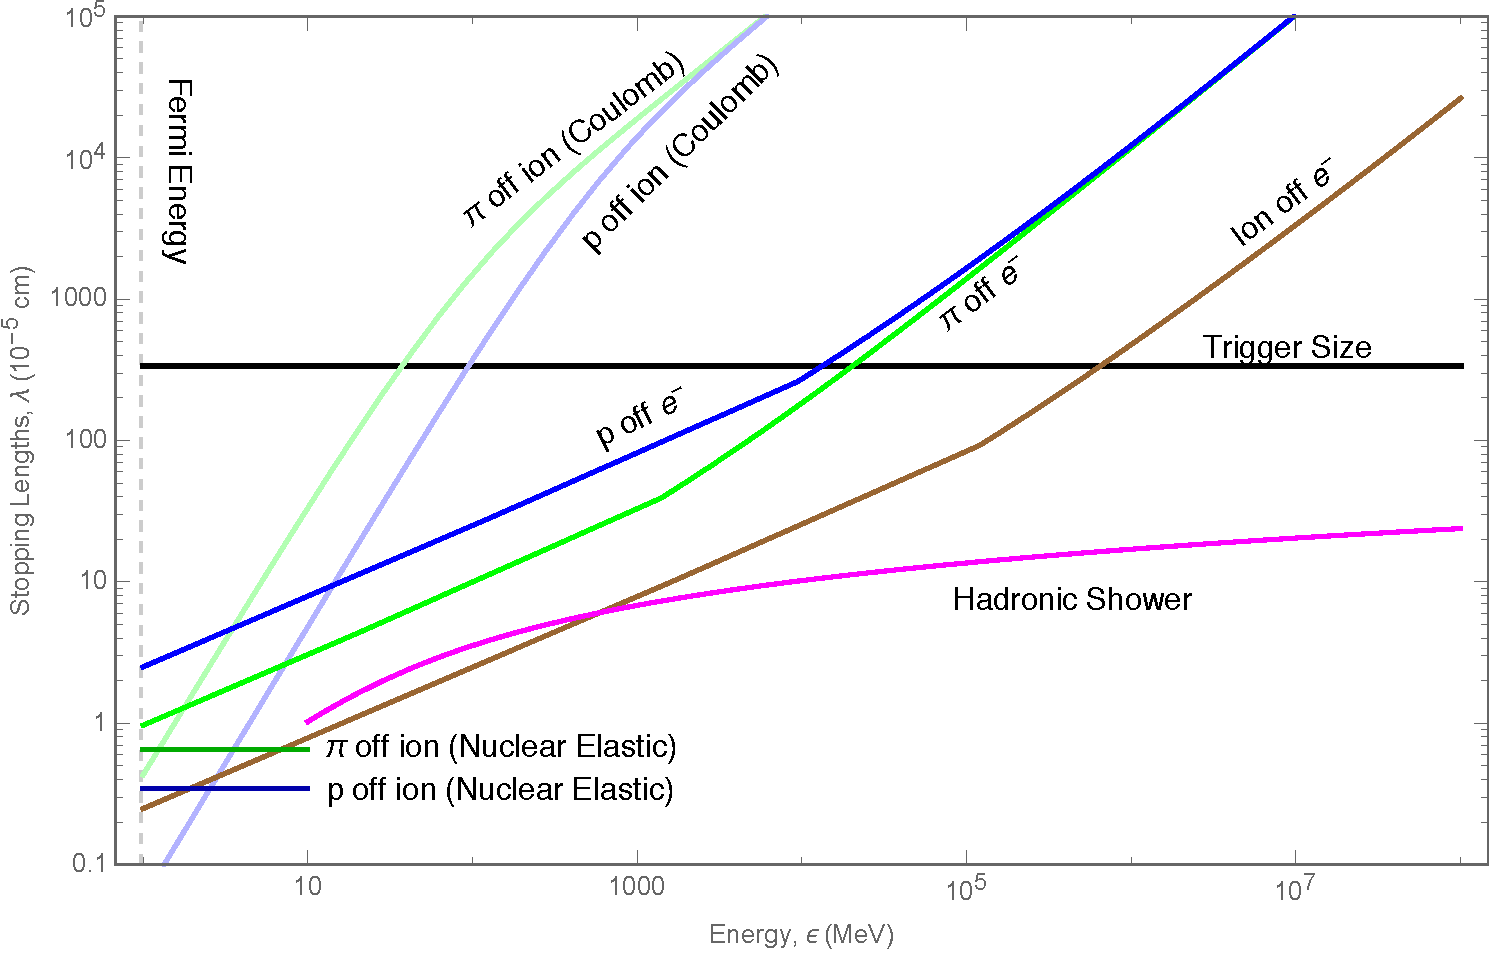
\includegraphics[scale=.3]{SPlowHad.pdf}
\caption{Stopping lengths for incident hadrons, plotted versus incident kinetic energy at low densities: $n_\text{ion}~\approx~10^{30}~\text{cm}^{-3}$, $M_\text{WD} \approx 0.85 M_{\astrosun}$. The magenta line is the hadronic shower length $X_\text{had}$.}
\label{fig:SPlowHad}
\end{figure}

\subsection{High-Energy Showers}

\paragraph{Hadronic Showers.}
Incident hadrons with kinetic energy $\epsilon$ larger than the nuclear binding scale $E_\text{nuc} \sim 10~\MeV$ will undergo violent inelastic collisions with carbon ions resulting in an $\OO(1)$ number of secondary hadrons.
This results in a roughly collinear shower of hadrons which ends when the constituents reach an energy $\sim E_\text{nuc}$.
This occurs over a shower length
\begin{align}
\label{eq:hadlength}
  X_\text{had} \sim l_\text{inel} \log\l\frac{\epsilon}{E_\text{nuc}}\r
  \approx 10^{-6} ~\text{cm} \l\frac{10^{32}~\text{cm}^{-3}}{n_\text{ion}}\r
\end{align}
where $l_\text{inel}$ is the mean free path for nuclear scatters, set by $\sigma_\text{inel} \approx 100 ~\text{mb}$, and we have taken the logarithm to be $\sim 10$.
The shower terminates into a cloud of $\sim 10~\MeV$ hadrons, composed of roughly equal fractions of pions, protons, and neutrons.
For a more detailed discussion of hadronic showers, see Appendix~\ref{sec:nuclear}.
Note that neutral pions of energy $10 - 100 ~\text{MeV}$ have a decay length to photons of $\delta_\pi \sim 10^{-6} ~\text{cm}$.
Hadronic showers will therefore generate an electromagnetic component carrying an $\OO(1)$ fraction of the energy.

\paragraph{Electromagnetic Showers.}
High-energy electrons and photons can also undergo radiative showers sustained by successive bremsstrahlung and pair-production events.
These terminate in a cloud of electrons and photons at some critical energy $E_\text{crit} \sim 100~\MeV$, set by the scale at which radiative processes become subdominant to elastic interactions.
Below this scale radiation can still be important, though EM showers do not occur.
Note that radiative processes are strictly forbidden for incident energies below the electron Fermi energy.

For sufficiently high energies, EM showers are elongated due to the ``Landau-Pomeranchuk-Migdal" (LPM) effect.
In a dense medium, arbitrarily soft virtual photons cannot be exchanged with only one ion, but rather interact simultaneously with multiple ions.
This generates an incoherence, suppressing the radiative cross-section above the LPM scale $E_\text{LPM}$ which scales inversely with medium density,
\begin{align}
    E_\text{LPM} \approx 1~\MeV
    \l \frac{10^{32}~\text{cm}^{-3}}{n_\text{ion}} \r
\end{align}
See Appendix~\ref{sec:emshowers} for more details.
At our highest densities EM showers are always LPM-suppressed, whereas at low densities we observe both regimes.
The corresponding shower lengths are
\begin{align}
  X_\text{EM} &\approx X_0 \cdot \begin{cases}
  \l \frac{\epsilon}{E_\text{LPM}} \r^{1/2} & \epsilon > E_\text{LPM} \\
  \;\;\;\;\;\, 1 & \epsilon < E_\text{LPM}
  \end{cases}
\end{align}
where
\begin{align}
  X_0 &\approx 10^{-7} ~\text{cm}
  \l\frac{10^{32}~\text{cm}^{-3}}{n_\text{ion}}\r
\end{align}
and are plotted in Figures \ref{fig:SPhighEM}, \ref{fig:SPlowEM} as the dashed bremsstrahlung/pair-production lines.
The energy scaling of LPM effect ensures that hadronic interactions dominate at sufficiently high energies even for electrons and photons.
At the highest densities, almost our entire energy range is LPM-suppressed, and EM showers only dominate for incident electrons and photons with energies between $ \sim 100 - 10^4~\text{MeV}$.
At low densities, EM showers provide the dominant stopping mechanism in the larger window $ \sim 100 - 10^6~\MeV$.

\paragraph{Photonuclear and Electronuclear Showers.}
Photons can interact hadronicly via quark-antiquark pairs and directly induce hadronic showers off ions.
The only quantitative difference between these showers and purely hadronic ones is that they require a slightly longer distance to initiate.
The initial photon-ion interaction is suppressed relative to the hadron-ion interaction by a factor of $\alpha$ required to produce a quark-antiquark pair.
This gives a photon range
\begin{align}
\label{eq:photonuclength}
  \lambda_{\gamma\text{-nuc}} \sim \frac{l_\text{inel}}{\alpha}
  \approx 10^{-5} ~\text{cm} \l\frac{10^{32}~\text{cm}^{-3}}{n_\text{ion}}\r.
\end{align}
Note that this is the distance to begin a hadronic shower, whereas the shower itself extends a distance $\sim X_\text{had}$.
The heating length $L_0$ (as used in Section~\ref{sec:Review}) is given by $\lambda_{\gamma\text{-nuc}} + X_\text{had}$ only if the DM produces many outgoing photons.
If a single high-energy photon is produced, $\lambda_{\gamma\text{-nuc}}$ only gives a displacement of the eventual heated region from the DM interaction vertex, while $L_0 \sim X_\text{had}$ will be set by the hadronic shower length.
In the purely hadronic case there is obviously no such hierarchy.

Electronuclear showers proceed analogously to photonuclear interactions.
High-energy electrons will radiate virtual photons that initiate hadronic showers.
This interaction is suppressed by an addition factor of $\alpha$ relative to the photonuclear processes, however a full calculation also yields an $\OO(10)$ logarithmic phase-space factor.
See Appendix~\ref{sec:nuclear} for details.
The electronuclear stopping length is
\begin{align}
\label{eq:electronuclength}
  \lambda_\text{e-nuc}
  \approx 10^{-4} ~\text{cm} \l\frac{10^{32}~\text{cm}^{-3}}{n_\text{ion}}\r.
\end{align}
This process differs qualitatively from the hadronic and photonuclear showers in that the original electron survives throughout the process.
Electronuclear stopping is best described as a continuous energy loss, as it is dominated by radiating $\sim 10~\MeV$ photons which initiate minimal hadronic showers.
The length scale of these showers is much less than the range of the electron $\lambda_\text{e-nuc}$.
The heating length due to high-energy electrons is thus given by $\lambda_\text{e-nuc}$ regardless of the number of electrons produced.

\paragraph{Neutrino-induced Showers.}
Neutrinos will scatter off ions with a cross section that increases with energy.
In these interaction, an $\OO(1)$ fraction of the neutrino energy is transferred to the nucleus with the rest going to produced electrons \cite{Formaggio:2013kya}---this is sufficient to start a hadronic shower.
At an energy of $\sim 10^{11} ~\GeV$, \cite{Formaggio:2013kya} calculates the neutrino-nuclear cross section $\sigma_{\nu-\text{nuc}} \sim 10^{-32} ~\cm^2$, which we will conservatively take as an estimate for even higher energies.
This gives length of $X_\nu \sim \text{meter}$ to initiate a shower.
While this is too large to provide heating via the release of many low-energy neutrinos, a single neutrino of energy $\sim \Eboom$ is indeed explosive.


\subsection{Low-Energy Elastic Heating}

The showering processes described above conclude with a cloud of $\sim 10~\MeV$ neutrons, protons, and charged pions or $\sim 100~\MeV$ electrons and photons.
Of course, particles at these energies may also be directly produced by the DM.
In this regime, Coulomb, Compton, and elastic nuclear scatters are the dominant processes, and eventually lead to thermaliation of ions.
The stopping powers for these processes are calculated in Appendix~\ref{sec:coulomb_ion},~\ref{sec:coulomb_elec}, and~\ref{sec:compton}.

\paragraph{Ions are a Leaky Bucket.}
We first note that heating ions to a temperature $\gtrsim T_F$ over a size $\gtrsim \lambda_T$ necessarily also heats the WD electrons and photons in that region.
Carbon ions themselves rapidly lose energy to cold electrons via Coulomb interactions, which in turn radiate photons that thermalize with other electrons via Compton scatters.
The range of ions is given in Figures~\ref{fig:SPlowHad} and~\ref{fig:SPhighHad} and that of electron bremsstrahlung and Compton scattering in Figures~\ref{fig:SPlowEM} and~\ref{fig:SPhighEM}. Note these are all below the trigger size at energies $~\MeV$.
Note one subtlety here: electron bremsstrahlung has a hard cutoff at the electron Fermi energy, which is possibly greater than the heated ion temperature $T \gtrsim \MeV$.
However, after the ions warm the degenerate electron gas to temperature $T$, there will be a thermal population of electrons carrying energy $E \sim E_F + T$ that are able to radiate photons of energies up to $k\sim T$, and thus still thermalize photons.

We therefore see that any processes which heats ions also establishes a hot EM bath.
What remains to check, however, is the length scale this EM bath.
This may nominally depend on the species and energy of the initial SM particles responsible for the heating, though we will show below that the heating length is always smaller or of order the trigger size for the species we consider.

\paragraph{Nucleons and Pions.}
Neutrons and neutral pions are the simplest species we consider, interacting at these energies only via elastic nuclear scatters with $\sigma_\text{el} \approx 1 ~\text{b}$.
% These are stronger than the inelastic interactions.
However, the mass hierarchy between these particles and ions will require $N \sim 10 - 100$ scatters to transfer the hadron's energy, which elongates the range by a random-walk factor $\sqrt{N}$.
This range is computed in Appendix~\ref{sec:nuclear} to be
\begin{align}
 \lambda_\text{el} &\approx
 10^{-7} ~\text{cm} \l\frac{10^{32}~\text{cm}^{-3}}{n_\text{ion}}\r,
\end{align}
which is always less than the trigger size.
Note that this may or may not be shorter than the $\pi^0$ decay length $\delta_\pi \sim 10^{-6} ~\text{cm}$, depending on the WD density.
Low-energy neutrons thus always provide efficient heating, low-energy neutral pions provide efficient heating at high densities, and the efficiency of neutral pions at low densities depends on the heating efficiency of $\sim 70~\text{MeV}$ photons.

Charged hadrons are subject to Coulomb interactions with ions and electrons, as well as nuclear scatters similar to their neutral brethren.
These ranges are plotted in Figures~\ref{fig:SPlowHad} and~\ref{fig:SPhighHad}.
It is curious that for $E \lesssim 10~\MeV$ scattering off electrons proves the least dominant of these processes, contrary to the behavior of terrestrial detectors.
This is due to significant Pauli-suppression of electron interactions at these energies, since $E_F \sim 1-10~\MeV$.
Low-energy charged hadrons will thus predominantly transfer energy to ions, which occurs below the trigger size for both nuclear-dominated and EM-dominated stopping.

In the context of a hadronic shower, the final-state hadrons are $\sim10~\MeV$ nucleons and pions, with each species carrying an $\OO(1)$ fraction of the initial energy.
These products will thermalize within a trigger size and thus hadronic showers are also an efficient heating mechanism.

\paragraph{Electrons and Photons.}
As shown in  Figures \ref{fig:SPhighEM} and \ref{fig:SPlowEM}, electron stopping at low energy is dominated by bremsstrahlung and photon stopping by Compton scatters.
Thus, at these energies electrons and photons first thermalize into an EM gas with size $\lambda_\text{brem} < \lambda_T$.
This gas cools and diffuses to larger length scales, eventually allowing subdominant processes to thermalize carbon ions.
The details of this evolution depend on the initial EM gas temperature, which is set by the total SM energy released by the DM.

If the gas remains above $T\sim10~\MeV$ by the time it has diffused to a scale $\lambda_{\gamma-\text{nuc}}$, it will begin a phase of photonuclear showers.
These will transfer an $\OO(1)$ fraction of energy into neutrons and other hadrons, which as discussed above will efficiency heat ions.
This heating will extend over the scale $\lambda_{\gamma-\text{nuc}}$ needed to begin photonuclear showers, which is indeed below the trigger size.

If the temperature falls below $10~\MeV$ before the photonuclear scale, the dominant process will be Coulomb scattering of hot electrons off WD ions.
Note that for the most dense WDs, the electron Fermi energy is $E_F \sim 10~\MeV$. At temperatures $T\lesssim E_F$, the electrons are partially degenerate and heating proceeds via the thermal tail with kinetic energies $\epsilon \sim E_F + T$.
(Note that the stopping length plots are plotted according to kinetic energy $\epsilon$.)
This range is plotted in Figures~\ref{fig:SPhighEM} and~\ref{fig:SPlowEM}, where it is seen that for EM gas temperatures $1-10~\MeV$ the electrons thermalize over a distance of order the trigger size.
The fact that this length scale is slightly larger than the trigger size simply means that constraints relying on this heating mechanism will have some volume dilution, increasing the necessary energy deposit according to~\eqref{eq:energy_boom_condition}.

In the context of EM showers terminating at $E_\text{crit}\sim100~\MeV$, the final-state electrons and photons will establish an EM gas of initial temperature $T \lesssim E_\text{crit}$ with length scale $\lambda_\text{brem}$.
At these temperatures the heat capacity is dominated by photons, so diffusion out to $\lambda_{\gamma-\text{nuc}}$ dilutes the temperature to $T \lesssim (\lambda_\text{brem} / \lambda_{\gamma-\text{nuc}})^{3/4} E_\text{crit}$.
Inspecting Figures~\ref{fig:SPhighEM} and~\ref{fig:SPlowEM} near $E_\text{crit}$, we find at high and low densities respectively $\lambda_\text{brem} / \lambda_{\gamma-\text{nuc}} \sim 10^{-1}$ and~$10^{-2}$.
The final temperatures at the photonuclear scale are thus $T \lesssim 20~\text{MeV}$ and $T \lesssim 3~\text{MeV}$ respectively.
This barely allows photonuclear showers at high density, and so we conservatively take EM shower products to thermalize ions through Coulomb interactions.

\section{Dark Matter-Induced Ignition}
\label{sec:DMexplode}

The unknown physics of DM sets the rate of SM particle production within the star as well as the initial distribution in space, momentum, and species of the products.
This information is needed to determine if a given DM encounter with a WD results in runaway fusion and with what frequency.
Of course, this can be done precisely for a specific DM model.
In this Section, we describe several general, illustrative classes of DM-WD encounters which demonstrate the explosiveness of ultra-heavy DM interactions.
We also calculate the typical rates at which these events take place in a WD.

\subsection{Classifying DM-WD Encounters}

DM can generically heat the WD medium through the three schematic interactions depicted in Figure \ref{fig:feynman}: DM-DM collisions, DM decays, and DM-SM scattering.
Note that for ultra-heavy DM these can be complicated events involving many (possibly dark) final states, analogous to the interactions of heavy nuclei.
We classify DM candidates into three types according to the interaction that provides the dominant source of heating, and refer to these as collision, decay, and transit candidates.
We additionally make simplifying assumptions about the spatial extent of these interactions.
For collisions and decays, we consider only ``point-like" heating events with all SM products produced in a localized region (smaller than the trigger size).
For transits, we consider only soft DM-SM scatters that result in a continuous release of particles along the DM trajectory.

We can also classify candidates according to the evolution of the DM itself inside the star.
Generally there will be some loss of DM kinetic energy due to DM-SM scatters---this is either incidental to the eventual heating of the star or represents the dominant heating mechanism.
We consider two simple, limiting cases depending on the magnitude of this energy loss relative to the DM kinetic energy: ``DM wind" and ``DM capture".
In the DM wind scenario, there is negligible energy loss and the DM simply passes through the star.
In the DM capture scenario, the energy loss due to DM-SM scatters is not capable of igniting runaway but is sufficient to stop the DM and cause it to accumulate inside the star.
We consider both scenarios for collision and decay candidates, for which the capture results in a significantly enhanced rate of events.
For simplicity we consider only the wind scenario for transit candidates, though an enhanced explosiveness from slowed DM continuously scattering off stellar constituents is certainly possible in some models.

\begin{figure}
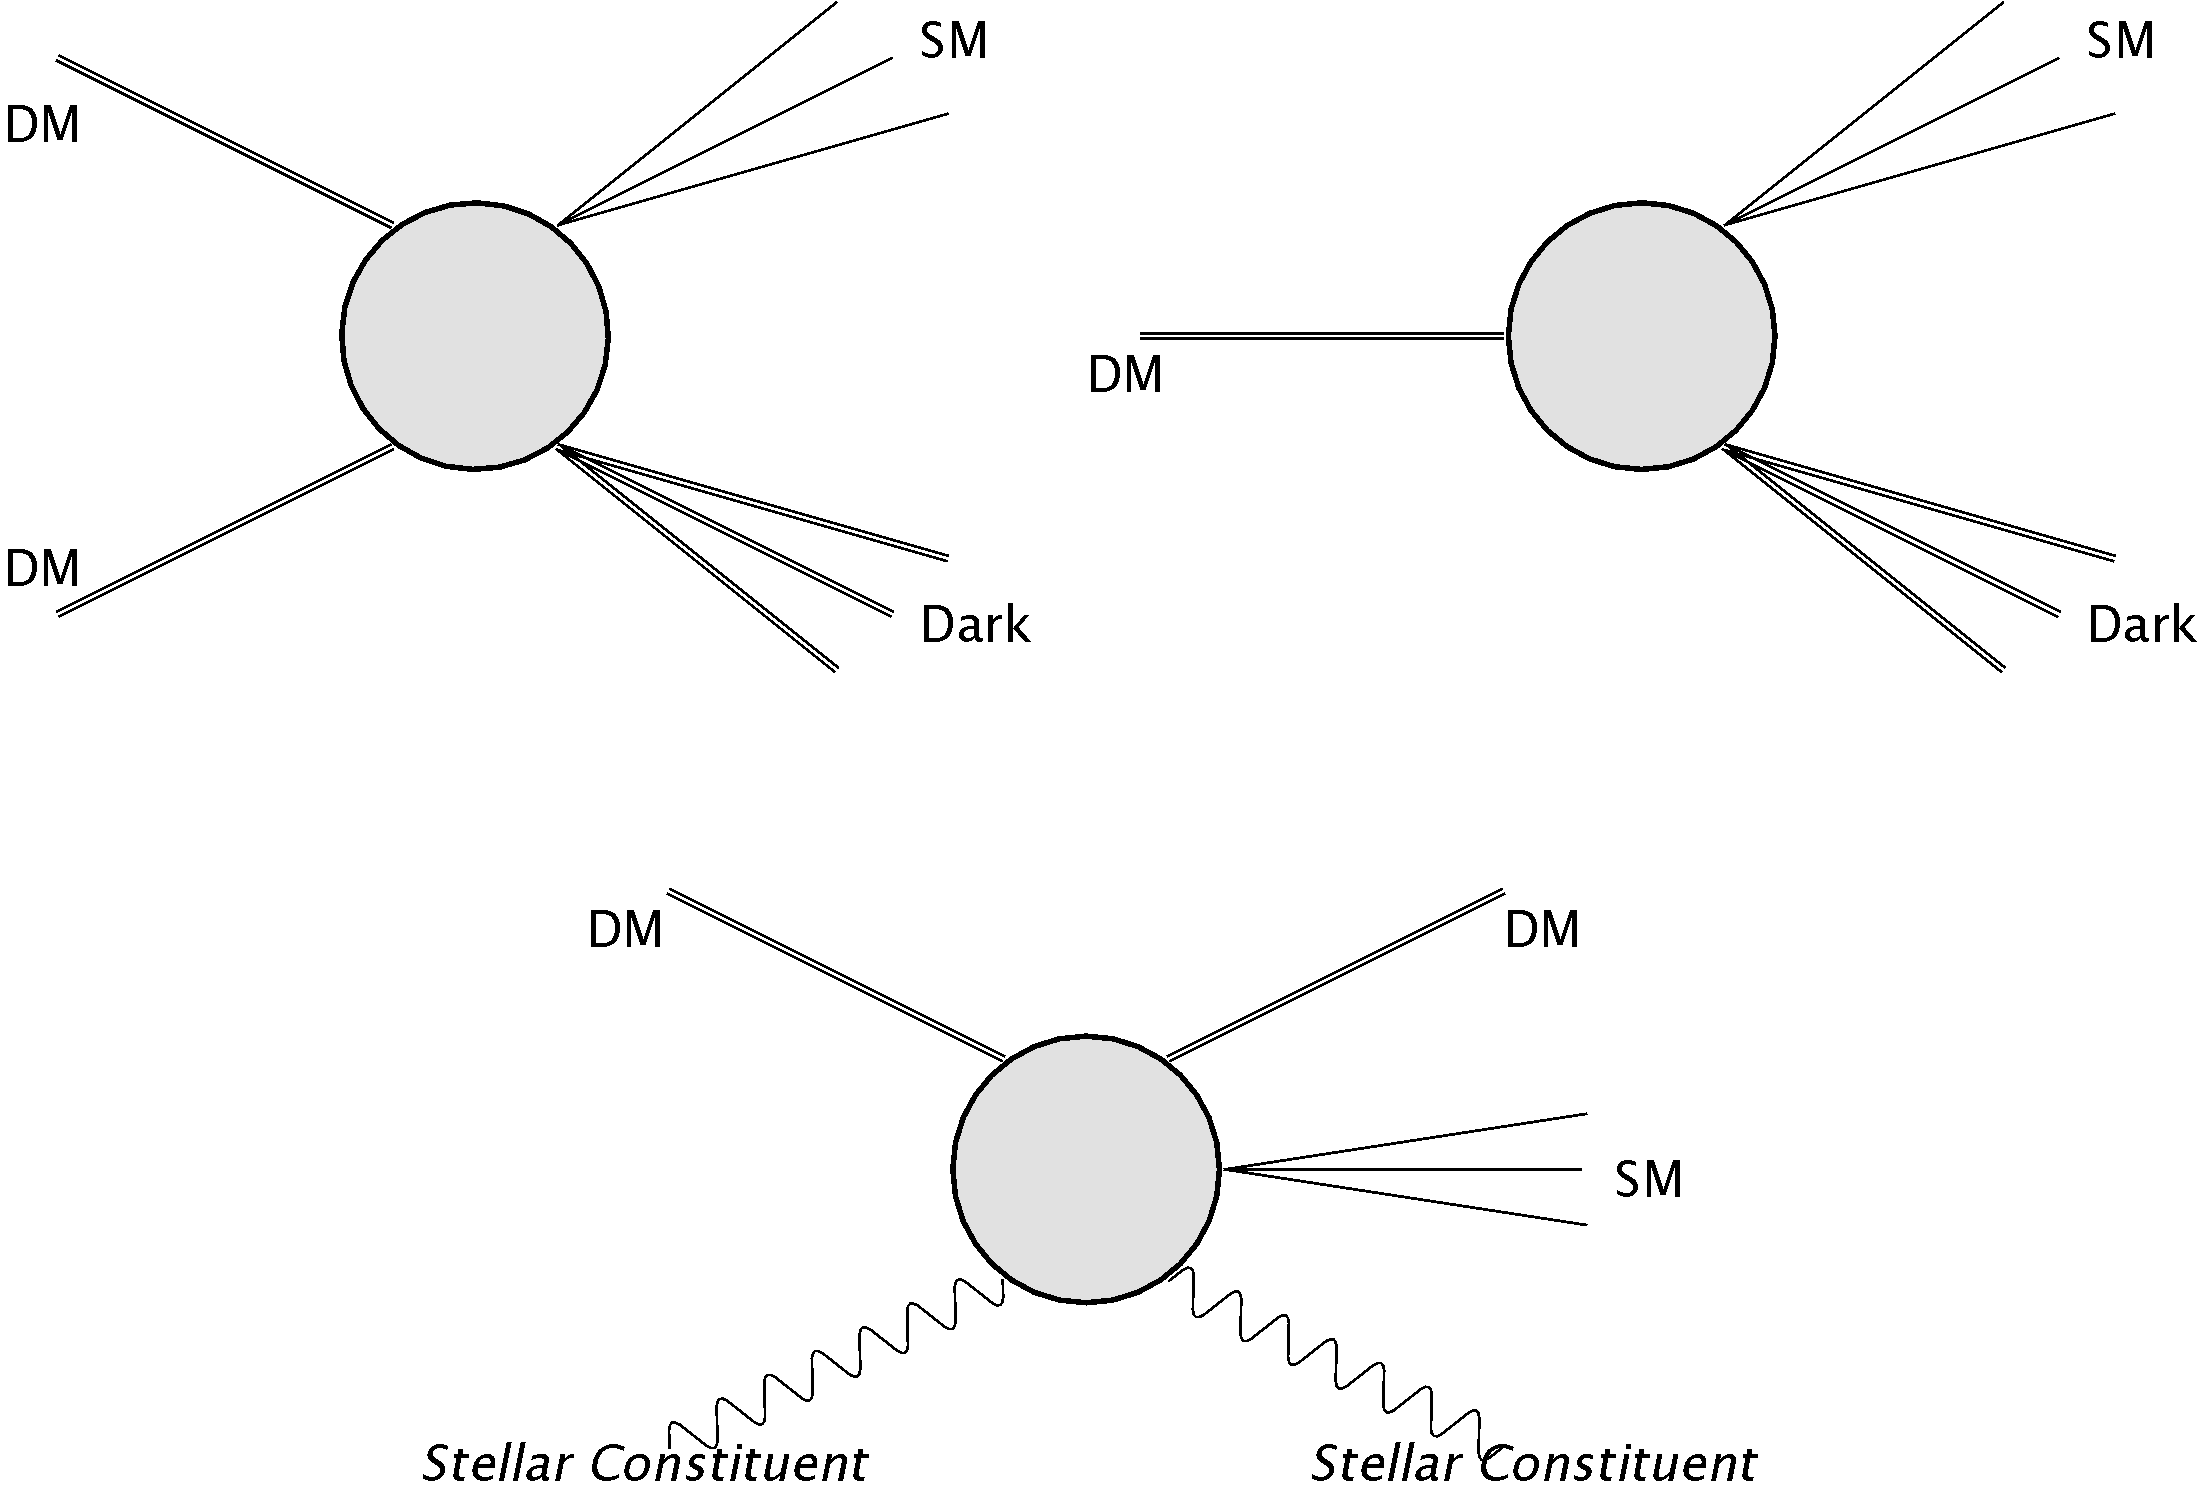
\includegraphics[scale=0.09]{feynman.png}
\caption{Schematic of possible non-gravitational DM interactions in a WD which release SM (and possibly dark sector) particles.}
\label{fig:feynman}
\end{figure}

\subsection{Transits}

\paragraph{Boom Condition.}
The energy deposited during a continuous heating event such as a DM transit is best described in terms of a linear energy transfer $(dE/dx)_\text{LET}$, the kinetic energy of SM particles produced per distance traveled by the DM.
If these products have a heating length $L_0$ then the relevant energy deposit must at minimum be taken as the energy transferred over the transit distance $L_0$.
Of course, we can always choose to consider energy deposits over a longer segment of the DM trajectory.
Importantly, as per the general condition \eqref{eq:energy_boom_condition} such a deposition is \emph{less} explosive unless $L_0$ is smaller than the trigger size $\lambda_T$.
Thus, we consider the energy deposited in a transit over the larger of these two length scales.
Assuming the energy of the DM is roughly constant over this heating event, the boom condition for transit heating is:
\begin{align}
\label{eq:transitexplosion}
  \left( \frac{d E}{d x} \right)_\text{LET} \gtrsim
  \frac{\Eboom}{\lambda_T} \cdot \text{Max}
  \left\{\frac{L_0}{\lambda_T}, 1 \right\}^2.
\end{align}

The above argument sums the individual energy deposits along the DM trajectory as though they are all deposited simultaneously.
This is possible if the DM moves sufficiently quickly so that this energy does not diffuse out of the region of interest before the DM has traversed the region.
We therefore require that the diffusion time $\tau_d$ across a heated region at temperature $T_f$ be larger than the DM crossing-time:
\begin{align}
  \tau_d \sim \frac{L^2}{\alpha(T_f)} \gg
  \frac{L}{v_\text{esc}},
\label{eq:SlowDiffusion}
\end{align}
where $\alpha(T)$ is the temperature-dependent diffusivity, and the DM transits at the stellar escape velocity $v_\text{esc} \approx 10^{-2}$.
This condition is more stringent for smaller regions, so we focus on the smallest region of interest, $L = \lambda_T$.
\eqref{eq:SlowDiffusion} is then equivalent to demanding that the escape speed is greater than the conductive speed of the fusion wave front, $v_\text{cond} \sim \alpha(T_f) / \lambda_T$.
Numerical calculations of $v_\text{cond}$ are tabulated in \cite{Woosley}, and indeed condition \eqref{eq:SlowDiffusion} is satisfied for all WD densities.

\paragraph{Event Rate: Wind Scenario.}
The rate of transit events is given by the flux of DM passing through a WD
\begin{align}
  \Gamma_\text{transit} \sim
  \frac{\rho_{\text{DM}}}{m_\text{DM}} R_\text{WD}^2
  \l\frac{v_\text{esc}}{v}\r v_\text{esc},
\label{eq:TransitFluxCondition}
\end{align}
where $m_\text{DM}$ is the DM mass, $\rho_\text{DM}$ is the local DM density near the WD, and $R_\text{WD} \approx 4000 ~\text{km}$ is the WD radius.
Here $v \sim 10^{-3}$ is galactic virial velocity, and the transit rate contains an $\OO(100)$ enhancement due to gravitational focusing.

\paragraph{WD Shielding.}
Runaway fusion only occurs in the degenerate WD interior where thermal expansion is suppressed as a cooling mechanism.
The outer layers of the WD, however, are composed of a non-degenerate gas and it is therefore essential that a DM candidate penetrate this layer in order to ignite a SN.
We parameterize this by a DM stopping power $(dE/dx)_\text{SP}$, the kinetic energy lost by the DM per distance traveled in the non-degenerate layer, and demand that
\begin{align}
\label{eq:CrustCondition}
  \left( \frac{d E}{d x} \right)_\text{SP} \ll
  \frac{m_\text{DM} v^2_\text{esc}}{R_\text{envelope}},
\end{align}
where $R_\text{envelope} \approx 50 ~\text{km}$ is the width of a WD envelope \cite{KippenhahnWeigert}.
Note that the DM stopping power in the non-degenerate layer $(dE/dx)_\text{SP}$ and the linear energy transfer in the degenerate interior $(dE/dx)_\text{LET}$ are possibly controlled by different physics and may have very different numerical values.
In addition, a transit heating event satisfying condition \eqref{eq:CrustCondition} will have negligible energy loss over the parametrically smaller trigger size or heating length $L_0$, validating the boom condition \eqref{eq:transitexplosion}.

\subsection{Collisions and Decays}

\paragraph{Boom Condition.}
For a point-like DM-DM collision or DM decay event releasing particles of heating length $L_0$, ignition will occur if the total energy in SM products satisfies condition~\eqref{eq:energy_boom_condition}.
Such an event will likely result in both SM and dark sector products, so we parameterize the resulting energy in SM particles as a fraction $f_\text{SM}$ of the DM mass.
For non-relativistic DM, the DM mass is the dominant source of energy and therefore $f_\text{SM} \lesssim 1$ regardless of the interaction details, although we may well suspect that $f_\text{SM} \ll 1$ for realistic models.
With this parameterization, the boom condition for both collisions and decays is
\begin{equation}
\label{eq:coldecay}
  m_\text{DM} f_\text{SM}  \gtrsim \Eboom \cdot \text{max} \left \{\frac{L_0}{\lambda_T}, 1 \right \}^3.
\end{equation}
We are thus sensitive to DM masses $m_\text{DM} \gtrsim 10^{16} ~\GeV$.

\paragraph{Event Rate: DM Wind.}
DM with negligible energy loss in the WD medium will traverse the star in roughly a time $\sim R_\text{WD}/v_\text{esc} \approx 0.1 ~\text{s}$ and have a number density within the WD enhanced relative to the galactic density by a factor $v_\text{esc}/v \sim \OO(10)$.
In the wind scenario, the DM-DM collision rate inside the WD parameterized by a cross-section $\sigma_\text{DM-DM}$ is:
\begin{align}
  \Gamma_\text{collision}
  %&\sim n_\text{DM} \sigma_\text{DM-DM} v_\text{esc} \cdot n_\text{DM} R_\text{WD}^3 \\
  \sim \l \frac{\rho_\text{DM}}{m_\text{DM}} \r^2 \sigma_\text{DM-DM} \l \frac{v_\text{esc}}{v}\r^2 v_\text{esc} R_\text{WD}^3.
  \label{eq:collisionDM}
\end{align}
Similarly the net DM decay rate inside the WD parameterized by a lifetime $\tau_\text{DM}$ is:
\begin{align}
 \Gamma_\text{decay}
  %&\sim \frac{1}{\tau_\text{DM}} \cdot n_\text{DM} R_\text{WD}^3 \\
  \sim \frac{1}{\tau_\text{DM}} \frac{\rho_{\text{DM}}}{m_\text{DM}} \l \frac{v_\text{esc}}{v}\r R_\text{WD}^3.
  \label{eq:decayDM}
\end{align}

\paragraph{Event Rate: DM Capture.}
We first review the evolution of DM within the star during a capture scenario.
As the DM rapidly loses energy it will thermalize with the star and slow to a velocity
\begin{equation}
v_\text{th} \sim \sqrt{\frac{T}{m_\text{DM}}} \approx 10^{-12} \l \frac{10^{16} ~\GeV}{m_\text{DM}}\r^{1/2},
\end{equation}
where $T \sim \keV$ is the WD temperature.
It will then accumulate at the virial radius set by $v_\text{th}$
\begin{align}
  R_\text{vir} &\sim \l \frac{T}{G m_\text{DM} \rho_\text{WD}}\r^{1/2} \\
  &\approx 0.1 ~\text{cm} \l \frac{10^{16} ~\GeV}{m_\text{DM}}\r^{1/2}
  \l \frac{10^{31} ~\cm^{-3}}{n_\text{ion}}\r^{1/2}, \nonumber
\end{align}
where we have assumed a constant WD density $\rho_\text{WD}$ within $R_\text{vir}$.
DM will collect at this radius until its total mass exceeds the WD mass within $R_\text{vir}$,
\begin{align}
    M_\text{core} &\sim \rho_\text{WD} R^3_\text{vir} \\
    &\approx 10^{29}~\GeV ~\l \frac{10^{16} ~\GeV}{m_\text{DM}}\r^{3/2}
  \l \frac{10^{31} ~\cm^{-3}}{n_\text{ion}}\r^{1/2}. \nonumber
\end{align}
The DM cloud will then begin gravitational collapse.
The exact nature of this collapse is model-dependent, eventually being arrested by DM-DM interactions or the formation of a black hole.
For composite DM, it is reasonable to suspect that the collapse stabilizes into a core of radius $R_\text{sta}$ larger than the Schwarzschild radius $\sim G M_\text{core}$.

There are several timescales relevant to this process.
The longest one is simply the time required for thermalized DM to drift down to the central core
\begin{align}
\label{eq:tdrift}
  t_\text{drift} &\sim \frac{R_\text{WD}}{v_\text{th}} \\
  &\approx 50 ~\text{yr} ~ \l \frac{m_\text{DM}}{10^{16} ~\GeV} \r^{1/2}. \nonumber
\end{align}
This is much larger than the time $t_\text{collect}$ needed for the star to collect a critical mass of DM or the timescale $t_\text{collapse}$ of the collapse itself. These times are given by
\begin{align}
\label{eq:tcol}
  t_\text{collect} &\sim \l \frac{M_\text{core}}{m_\text{DM}}\r \frac{1}{\Gamma_\text{transit}} \\
  & \approx 10 ~\text{s} \l \frac{10^{16} ~\GeV}{m_\text{DM}} \r^{3/2} \l \frac{0.4 ~\GeV/\text{cm}^3}{\rho_\text{DM}} \r,\nonumber
\end{align}
evaluated at $n_\text{ion} \sim 10^{31} ~\cm^{-3}$, and
\begin{align}
  t_\text{collapse} \sim \frac{R_\text{vir}}{v_\text{th}}
  \approx 3 ~\text{s} ~ \l \frac{10^{31} ~\cm^{-3}}{n_\text{ion}}\r^{1/2}
\end{align}
This expression for $t_\text{collapse}$ assumes the DM remains thermalized with the WD medium, but even if it is in complete gravitational free-fall there is only an $\mathcal{O}(1)$ speedup.
The core thus forms in a time $t_\text{drift}$, provided the mass of DM is sufficiently small---for masses $m_\text{DM} \gtrsim 10^{30}~\GeV$ the core will not form within the lifetime of the star.
Note that the collect time $t_\text{collect}$ \eqref{eq:tcol} has a non-trivial dependence on WD density: this is manifest in the values for $v_\text{esc}$ and $R_\text{WD}$.

For decay heating, capture gives an enhancement due to the increased number of DM particles within the WD.
This can be very large if the DM core admits decays, however it is still significantly enhanced over the wind scenario even for inert cores (as in the case that the DM forms a black hole).
We have an enhancement of the net decay rate \eqref{eq:decayDM} by a factor
\begin{align}
\label{eq:enhancedecay}
  \frac{v_\text{esc}}{v_\text{th}}
  \approx 10^{10} \l \frac{m_\text{DM}}{10^{16}~\GeV} \r^{1/2}
\end{align}
due to the increased time spent by the DM in the WD medium before joining the inert core.

In the case of DM-DM collision heating, it is possible that the collapse of the core will induce an ignition event due to the enhancement of DM number density during the collapse.
This would set the lifetime of WDs to $t_\text{collect}$.
During the collapse, the rate of collisions taking place at a radius $r$ within the enclosed volume is given by
\begin{align}
\Gamma_\text{collision}(r) \sim \l \frac{M_\text{core}}{m_\text{DM}} \r^2 \frac{1}{r^3} \sigma_\text{DM-DM} v(r),
\end{align}
where $v(r)$ is the velocity of DM - this could be either free-fall velocity or $v_\text{th}$ if the DM remains thermalized.
Integrating to the stable radius $R_\text{sta}$, we find the total number of collisions during the collapse is
\begin{align}
  N_\text{col} \sim \l \frac{M_\text{core}}{m_\text{DM}} \r^2 \frac{\sigma_\text{DM-DM}}{R_\text{sta}^2}.
 \end{align}
Assuming the collapse proceeds until the DM core becomes a black hole, the number of collisions is
\begin{align}
  N_\text{col} \sim \frac{\sigma_\text{DM-DM}}{G^2 m_\text{DM}^2}.
 \end{align}
If the collapse itself is not explosive, there is still an enhanced collision rate relative to the wind scenario due to DM colliding while in-falling to the core.
Again we look at the conservative situation of an inert core - the rate is obviously much greater if the core is stabilized in a fluid state which admits DM-DM collisions.
The rate of in-falling collisions is enhanced over the wind collision rate \eqref{eq:collisionDM} by a factor
\begin{align}
\label{eq:enhancecollision}
   \frac{R_\text{WD}}{R_\text{sta}} \times \frac{v_\text{esc}}{v_\text{th}},
\end{align}
which again depends on the physics of $R_\text{sta}$.

\paragraph{Event Rate: DM Capture and Multiple Collisions}

Up until now, we only considered the case that a single DM-DM collision releases sufficient energy \eqref{eq:coldecay} in order to trigger runaway fusion.
However, the possibility of a DM core collapse in the star provides up an interesting alternative:

\section{Dark Matter Constraints}
\label{sec:Constraints}

We now constrain some simplified models of DM which will ignite a WD via one of the processes parameterized in Section \ref{sec:DMexplode}.
First, however, we review how WD observables constrain DM candidates capable of triggering SN.

\subsection{Review of WD Observables}
Following the discussion of \cite{Graham:2015apa}, our constraints come from (1)~the existence of heavy, long-lived white dwarfs, or (2)~the measured type Ia SN rate.
The typical age of a WD is of order the age of the universe $\sim \text{Gyr}$.
RX~J0648.04418 is a nearby star and one of the heavier known WDs, with a mass $\sim 1.25 ~M_{\odot}$ \cite{Mereghetti:2013nba} and local dark matter density which we will take to be $\rho_\text{DM} \sim 0.4 ~\GeV/\text{cm}^3$.
Of course, this is not the only known heavy WD---the Sloan Digital Sky Survey \cite{SDSS} has found $20+$ others.
 % https://heasarc.gsfc.nasa.gov/db-perl/W3Browse/w3hdprods.pl
The NuStar collaboration has also recently uncovered evidence for the likely existence of $\sim 1.25 ~M_{\odot}$ WDs in the galactic center \cite{NuStar}, where it is estimated that $\rho_\text{DM} \sim 10^3 ~\text{GeV}/\text{cm}^3$ \cite{Nesti:2013uwa}.
Such heavy candidates are particularly suited for our constraints as the energy deposit necessary to trigger SN $\Eboom$ is a decreasing function of WD mass.
However, less dense white dwarfs are significantly more abundant in the galaxy.
Thus, even if a sufficiently massive DM is unable to trigger a violent heating event within the lifetime of a WD, it could still ignite enough lighter WDs to affect the measured SN rate of $\sim $ 0.3 per century.
The DM-induced SN rate is estimated using the expected number of white dwarfs per galaxy $\sim 10^{10}$ and their mass distribution \cite{SDSS}.
Simulations indicate that only WD masses heavier than $\sim 0.85 ~M_{\odot}$ will result in optically visible SN \cite{Graham:2015apa}.
Therefore, most of the stars exploded in this manner will be in the mass range $\sim 0.85 - 1 ~M_{\odot}$, resulting in weaker SN than expected of typical Chandrasekhar mass WDs.

To summarize, a bound on DM parameters can be placed if either a single explosive event occurs during the lifetime of an observed star such as RX~J0648.04418, or the SN rate due to such DM events throughout the galaxy exceeds the measured value.
Note that for low-mass WDs dominated by photon diffusion, $\Eboom$ is a strong function of WD density.
In \cite{Graham:2015apa} the central WD density is used to constrain black hole transits with the justification that the density is nearly constant for much of the star.
The average density for WDs is typically a factor $\sim 10^{-2} - 10^{-1}$ less than the central density, although it is found that the WD density only changes by an $\OO(1)$ fraction from the central value up to a distance $\sim R_\text{WD}/2$ \cite{Chandrasekhar}.
Therefore the central density is a valid approximation as long as we consider heating events within this ``modified" WD volume.
For simplicity, we employ this approach.

\subsection{Transit Constraints}
\label{sec:TransitConstraints}

In order to constrain a DM model through its transit interaction with a WD, we require that it satisfy the boom condition \eqref{eq:transitexplosion}.
This is given in terms of an LET, which parameterizes the ability for DM to release sufficient energy to the star in the form of SM particles.
$(dE/dx)_\text{LET}$ for any realistic DM model would necessarily involve a sum over stellar targets along with species that could be produced, as well as an integral over the produced particle spectrum.
However, we will consider a simplified interaction in which $\sigma_{Ni\epsilon}$ denotes the cross-section for DM to scatter off a stellar constituent (e.g. ions), producing $N$ particles of SM species $i$ and individual energy $\epsilon$.
If this were the only available channel for the DM to deposit energy, then the LET could be written as
\begin{align}
\label{eq:schematicLET}
  \left( \frac{d E}{d x} \right)_\text{LET} = n_\text{ion} \sigma_{Ni\epsilon} N\epsilon.
\end{align}
The heating length for such a DM-SM scattering interaction is computed in Section~\ref{sec:SMHeating}.

Additionally, consider the case that the LET $(dE/dx)_\text{LET}$ and DM stopping power $(dE/dx)_\text{SP}$ are equal---that is, the DM loses kinetic energy at the same rate as energy is deposited to the WD.
While such a statement is certainly not true for all DM models (such as the Q-ball, which liberates binding energy rather than transferring kinetic energy), it provides a useful benchmark to express constraints.
It is interesting to note that in this case combining the transit explosion condition \eqref{eq:transitexplosion} with $\eqref{eq:schematicLET}$ yields a lower bound on DM mass such that the DM is able to both penetrate the envelope \emph{and} trigger an explosion:
\begin{align}
\label{eq:transitmass}
m_\text{DM} > \Eboom \l \frac{R_\text{envelope}}{\lambda_T} \r \l \frac{\rho_\text{envelope}}{\rho_\text{central}} \r \frac{1}{v_\text{esc}^2}.
\end{align}
For the typical parameters of a $1.25 ~M_{\odot}$ WD we find that the DM mass must be greater than $\sim 10^{28} ~\GeV$ to ensure a penetrating and explosive transit, taking the density of the WD envelope $\rho_\text{envelope}$ to be a nominal $\OO(10^{-3})$ fraction of the central density $\rho_\text{central}$~\cite{KippenhahnWeigert}.
In other words, if \eqref{eq:transitmass} were violated then the DM interaction is either not strong enough to ignite the WD or is so strong that the DM cannot penetrate the envelope without losing appreciable kinetic energy.
We reiterate, however, that this bound is only applicable when the energy input to the WD is chiefly coming from the DM kinetic energy, rather than binding energy or other sources.

With the above schematic for a DM transit, we use the rates and heating lengths computed in previous sections to constrain the parameter $\sigma_{Ni\epsilon}$ as a function of DM mass $m_\text{DM}$.
This is done in Figure \ref{fig:transitclasses} using the different classes of observation available and for representative choices of $\epsilon$ and SM species $i$ released.

\begin{figure}
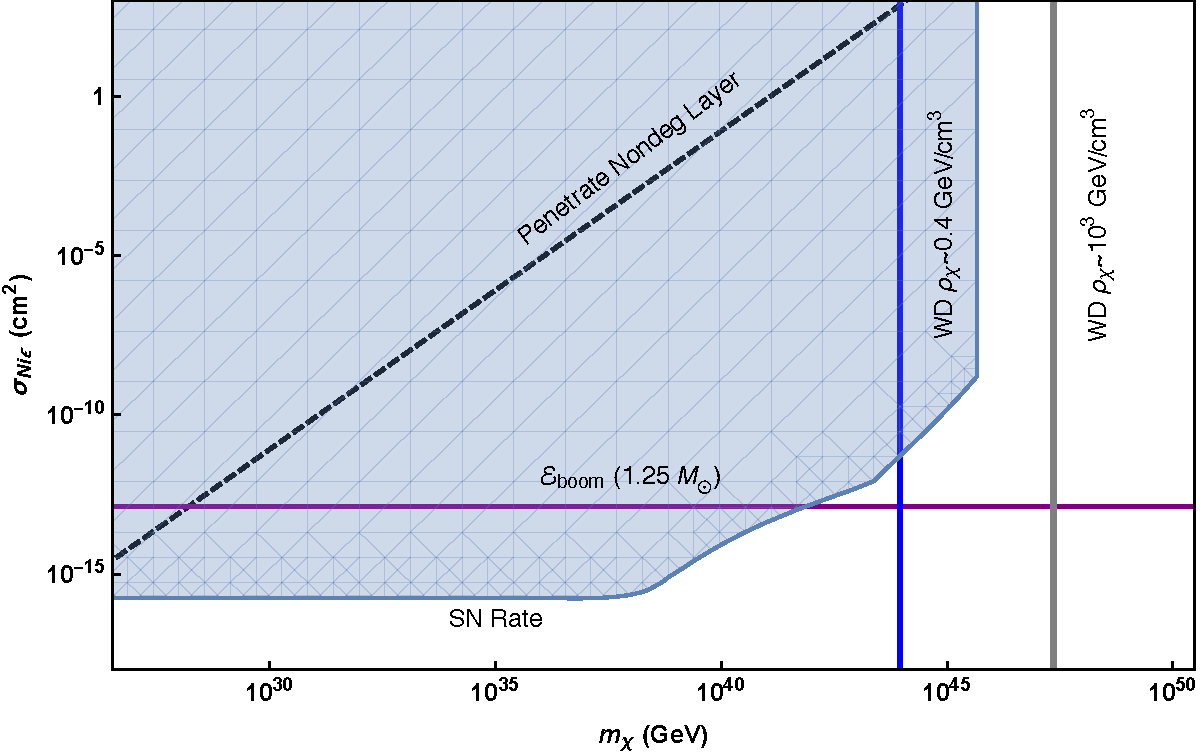
\includegraphics[scale=.45]{transitobservation.pdf}
\caption{Constraints on a DM-nuclei scattering cross-section to produce a single TeV photon. Bounds come from demanding that heating events satisfy \eqref{eq:transitexplosion} and occur at a rate \eqref{eq:TransitFluxCondition} rapid enough to either ignite a single observed $1.25~M_{\astrosun}$ WD in its lifetime (local and galactic center) or exceed the measured SN rate in our galaxy.}
\label{fig:transitclasses}
\end{figure}

\subsection{Collision and Decay Constraints}
\label{sec:CollisionConstraints}

In order to constrain a DM model through its annihilations or decays within a WD, we require that it satisfy the boom condition \eqref{eq:coldecay}.
Consider a simplified interaction where an annihilation or decay releases $N$ particles of SM species $i$ and individual energy $\epsilon$.
If we assume a fractional parameter $f_\text{SM}=1$, this corresponds to the entire mass of DM being converted into SM products $i$, each with energy $m_\text{DM}/N$.
These will deposit their energy and thermalize ions within a distance described in Section \ref{sec:SMHeating}.

With this schematic for DM-DM collisions, we use the rates and heating lengths computed in previous sections to constrain the cross section $\sigma_\text{DM-DM}$ as a function of $m_\text{DM}$ using the different classes of observation available and for representative choices of $f_\text{SM}$ and SM species $i$ released.
This is done in Figure \ref{fig:collisionclasses}.
In a similar manner, we constrain the lifetime $\tau_\text{DM}$ as a function of $m_\text{DM}$ in Figures \ref{fig:decayclasses}.
These plots both show constraints for the more straightforward ``wind'' scenario, as discussed in section~\ref{sec:DMexplode}.
In the ``capture'' scenario, constraints have the same qualitative shape but reach to much lower cross-sections and longer lifetimes.
In the extreme case that DM collapses to a black hole, we rule out lifetimes up to a factor of $10^{10}$ larger and cross-sections $10^{-40}$ smaller than in the ``wind'' scenario.

\emph{Complementary Limits}~~It is important to note that there are additional limits on DM interactions of this kind, complementary to the limits placed from WDs.
For instance, DM can annihilate or decay into ultra-high energy particles within our galactic halo and therefore contribute to the cosmic ray flux seen in terrestrial air shower detectors.
As cosmic rays of energy greater than $\sim 10^{12} ~\GeV$ have not yet been observed \cite{ThePierreAuger:2015rha, AbuZayyad:2012ru}, this places a concrete limit on DM interaction parameters $\sigma_\text{DM-DM}$ and $\tau_\text{DM}$ which involve the release of such ultra-high energy particles.
In theory, a constraint may also be placed on lower-energy SM products from DM annihilations or decays, which would provide an additional source for the measured cosmic ray flux, although such a detailed analysis is beyond the scope of this work.

The cosmic ray constraint on DM is derived by requiring that the expected time for an event to strike earth is less than the lifetime of the detector $\sim 10 ~\text{yr}$.
For a cosmic ray detector with area $ \sim (50~\text{km})^2$ \cite{ThePierreAuger:2015rha}, we find that the cosmic ray bounds are weaker than the WD bounds except in the DM decay ``wind scenario", where the cosmic rays bounds are comparable within a couple orders of magnitude to those due to the observation of a local WD.
This coincidence is simply a consequence of the similar ``space-time volumes" of the two systems.
A cosmic ray detector sees events within a space-time volume $\sim (R_\text{det}^2 R_\text{halo} \times 10 ~\text{yr})$ which is comparable to the WD space-time volume for decay events $\sim (R_\text{WD}^3 \times 10^9 ~\text{yr}\times 10)$, including the factor of 10 gravitational enhancement.

In addition, there are various cosmological bounds on DM interactions.
By requiring that the galactic halo has not diminished by more than an $\OO(1)$ factor during its lifetime, we constrain $\sigma_\text{DM-DM}/m_\text{DM} \lesssim \text{barn}/\GeV$, regardless of the precise details of the collision.
This is similar in magnitude to the DM self-interaction bounds from colliding galaxy clusters \cite{Randall:2007ph}.
The cosmological bound on DM lifetime $\tau_\text{DM} \gtrsim 100 ~\text{Gyr}$ is also independent of the nature of the decay products (see \cite{Poulin:2016nat} for details).
Since the limits imposed by the WD scale as $\sigma_\text{DM-DM} \propto m_\text{DM}^2$ and $\tau_\text{DM} \propto m_\text{DM}^{-1}$, there will necessarily be a sufficiently large DM mass for which the above cosmological considerations are the more stringent constraints on its interactions.
This occurs for DM masses $m_\text{DM} \sim 10^{25} - 10^{30} ~\GeV$.


\begin{figure}
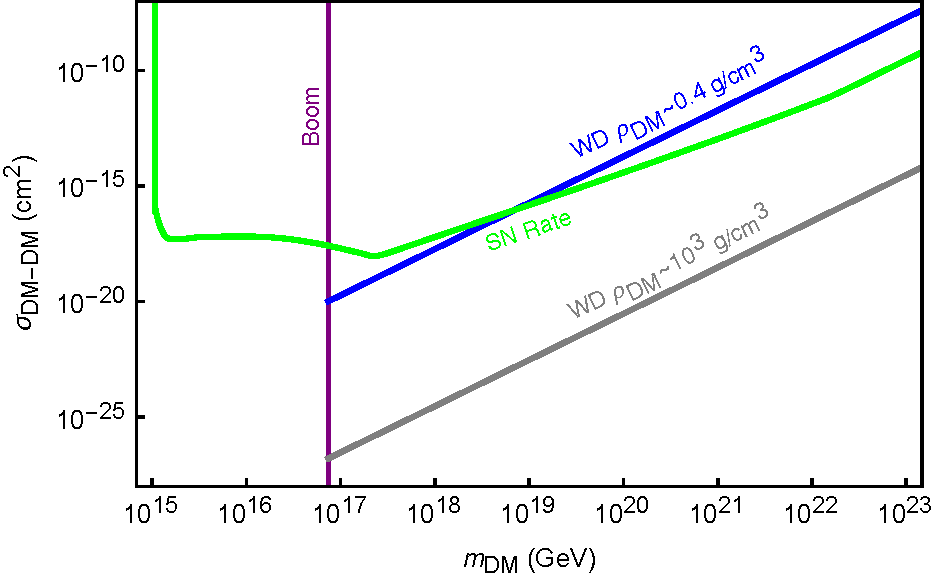
\includegraphics[scale=.45]{collisionobservation.pdf}
\caption{Constraints on DM-DM collision cross-section into photons with individual energy $\epsilon > 10~\text{MeV}$ and $f_\text{SM} = 1$. Bounds come demanding that heating events satisfy \eqref{eq:coldecay} and occur at a rate \eqref{eq:collisionDM} (``wind scenario'') rapid enough to either ignite a single observed $1.25~M_{\astrosun}$ WD in its lifetime (local and galactic center) or exceed the measured SN rate in our galaxy.  In the ``capture'' scenario, constraints are of a similar shape but reach to cross-sections of $\sim 10^{-47}~\cm^2$ for maximal collapse.}
\label{fig:collisionclasses}
\end{figure}

\begin{figure}
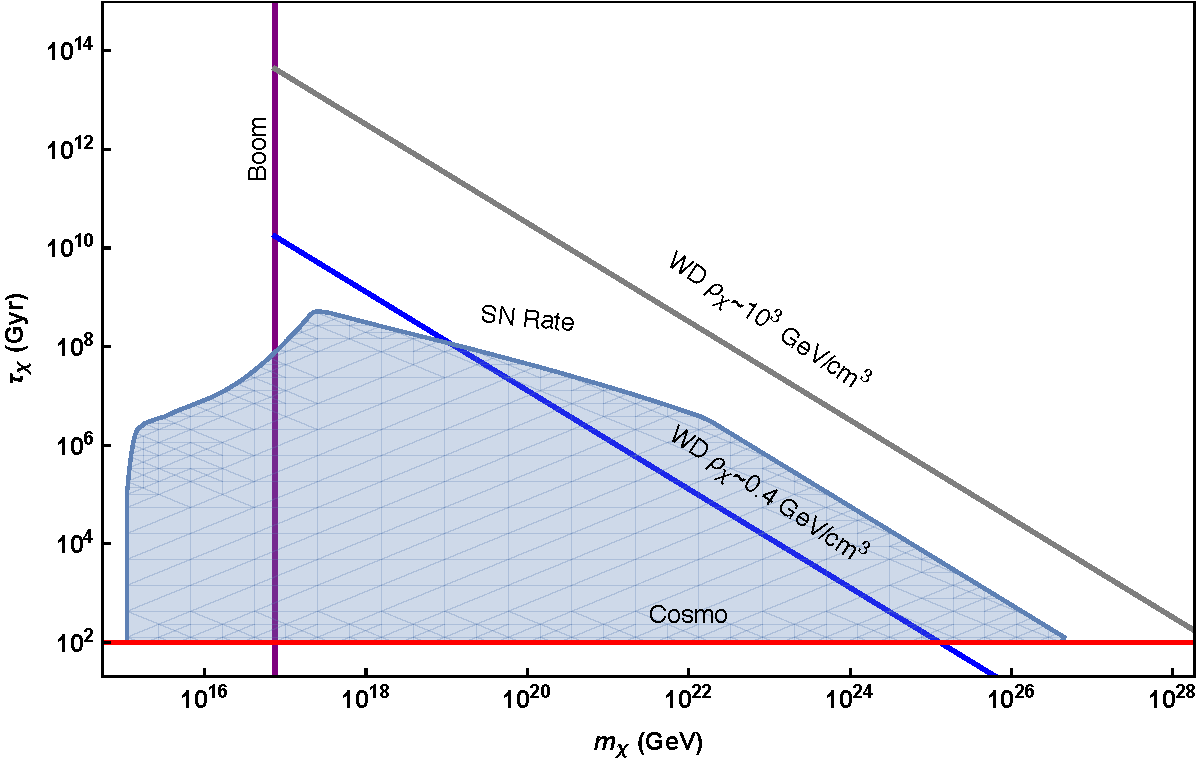
\includegraphics[scale=.45]{decayobservation.pdf}
\caption{Constraints on DM decay lifetime into photons with individual energy $\epsilon > 10~\text{MeV}$ and $f_\text{SM} = 1$. Bounds come demanding that heating events satisfy \eqref{eq:coldecay} and occur at a rate \eqref{eq:decayDM} (``wind scenario'') rapid enough to either ignite a single observed $1.25~M_{\astrosun}$ WD in its lifetime (local and galactic center) or exceed the measured SN rate in our galaxy. In the ``capture'' scenario, constraints are of a similar shape but reach to lifetimes of $10^{18}~\text{Gyr}$ for maximal collapse.}
\label{fig:decayclasses}
\end{figure}

\section{Q-balls}
\label{sec:QBalls}

Having derived constraints on generic models of ultra-heavy DM, we turn towards a concrete example.
In various supersymmetric extensions of the SM, non-topological solitons called Q-balls can be produced in the early universe \cite{Coleman:1985ki, Kusenko:1997si}.
If these Q-balls were stable, they would comprise a component of the DM today.
For gauge-mediated models with flat scalar potentials, the Q-ball mass and radius are given by
\begin{equation}
\label{eq:Qballprop}
M_Q \sim m_S Q^{3/4}, ~~~ R_Q \sim m_S^{-1} Q^{1/4},
\end{equation}
where $m_S$ is related to the scale of supersymmetry breaking, and $Q$ is the global charge of the Q-ball---in our case, baryon number.
The condition $M_Q/Q < m_p$ ensures that the Q-ball is stable against decay to nucleons.
When an electrically neutral baryonic Q-ball interacts with a nucleon, it absorbs its baryonic charge and induces the dissociation of the nucleon into free quarks.
During this proton decay-like process, $\sim \text{GeV}$ of energy is released through the emission of 2--3 pions~\cite{Kusenko:1998}.
We assume that for each Q-ball collision, there is equal probability to produce $\pi^0$ and $\pi^\pm$ under the constraint of charge conservation.
Note that a sufficiently massive Q-ball will become a black hole if $R_Q \lesssim G M_Q$.
In the model described above, this translates into a condition $(M_\text{pl}/m_S)^4 \lesssim Q$.

We now determine the explosiveness of a Q-ball transit.
As in Section \ref{sec:Constraints}, this process is described by the parameter
\begin{equation}
\label{eq:QballLET}
\l\frac{dE}{dx}\r_\text{LET} \sim n_\text{ion} \sigma_Q N \epsilon,
\end{equation}
where the nuclear collision results in $N \sim 30$ pions released, each with kinetic energy $\epsilon \sim 500 ~\text{MeV}$.
These pions induce hadronic showers which terminate in low-energy hadrons that rapidly transfer their energy to ions via elastic scatters, as discussed in Section~\ref{sec:SMHeating}.
Thus the Q-ball transit has a heating length within the trigger size, and the Q-ball cross-section necessary to trigger runaway fusion is given by equations~\eqref{eq:transitexplosion} and~\eqref{eq:QballLET}:
\begin{equation}
 \sigma_Q \gtrsim \frac{1}{n_\text{ion}} \frac{\Eboom}{\lambda_T}
 \l \frac{1}{10~\GeV} \r.
\end{equation}
We see $\sigma_Q \approx 10^{-12} ~\text{cm}^2$ is sufficient to blow up a $\sim 1.25 ~M_{\odot}$ WD.
The cross-section for this interaction is approximately geometric
\begin{align}
\sigma_Q \sim \pi R_Q^2,
\end{align}
and so $Q \gtrsim 10^{42} ~(m_S/\text{TeV})^4$ can be adequately constrained from the observation of a single, heavy WD.
Note that the Q-ball interaction described above results in minimal slowing or transfer of kinetic energy for Q-balls this massive, so transits will easily penetrate the non-degenerate WD layer \eqref{eq:CrustCondition}.

The strongest previous constraints on Q-balls come from Super-Kamiokande as well as air fluorescence detectors of cosmic rays \cite{Dine:2003ax}.
However, the constraints due to white dwarfs are in a fundamentally complementary region of parameter space.
These are plotted in Figure~\ref{fig:Qballconstraint}.
As a comparison, the combined limits from Super-K and the OA, TA cosmic ray detectors are shown in red.
We have also included the constraints from a WD which result from considering gravitational heating during a Q-ball transit, as in \cite{Graham:2015apa}.

\begin{figure}
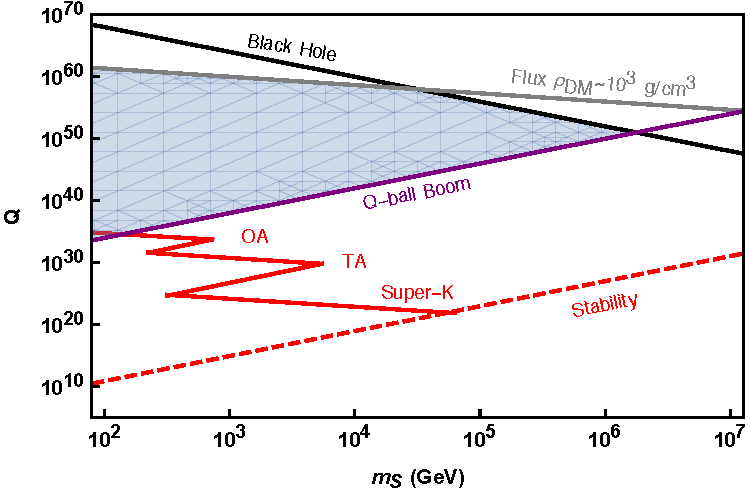
\includegraphics[scale=.3]{Qballconstraint.pdf}
\caption{Constraints on baryonic Q-balls from transits of a $\sim 1.25 ~M_{\odot}$ WD in the galactic center, $\rho_\text{DM} \sim 10^3 ~\text{g}/\text{cm}^3$.
We include constraints from heating by strong interactions with nuclei and gravitational interactions (dynamical friction).
Also shown are the limits from Super-K and the OA, TA cosmic ray detectors, extracted from \cite{Dine:2003ax}.}
\label{fig:Qballconstraint}
\end{figure}

\section{Discussion}
\label{sec:Discussion}

The detection of ultra-heavy DM is an open problem which will likely require a confluence of astrophysical probes.
Here we present a comprehensive guide to containing these DM candidates through annihilates, decays, and transits within a WD that release sufficient SM energy to trigger a type Ia supernova.
In particular, we calculate the energy loss of high-energy particles due to SM interactions within the WD medium and determine the conditions for which a general energy deposition will heat a WD and ignite thermonuclear runaway.
The formalism provided will enable WDs to be applied as detectors for any DM models capable of heating the star through non-gravitational interactions, and as a concrete example we are able to place bounds on supersymmetric Q-ball DM over a wide region of parameter space.

In general, the phenomenology of such a DM-induced event will be the ignition of sub-Chandrasekhar mass progenitors.
This raises the tantalizing possibility that DM encounters with a WD can act as an alternative explosion mechanism and progenitor system for type Ia SN.
For decades, standard lore has been that type Ia SN are caused by accretion onto carbon-oxygen white dwarfs in binary systems that reach the critical $\sim 1.4 ~M_{\odot}$ Chandrasekhar mass limit.
Nevertheless, it is well-known that such a mechanism cannot account for all observed type Ia SN.
Recent observations \cite{Scalzo:2014sap, Scalzo:2014wxa} suggest that an $\OO(1)$ fraction of the observed type Ia SN appear to have sub-Chandrasekhar progenitors.
A leading explanation for this phenomenon is the detonation of a surface layer of helium which drives a shock into the interior of a sub-Chandrasekhar-mass WD \cite{Woosley1994,Fink:2007fv}.
However, in light of the lack of understanding of DM and its interactions, it is worthwhile to consider whether a DM-WD encounter may also give rise to type Ia SN progenitor.

\begin{appendices}

\section{Particle Stopping in a White Dwarf}
\label{sec:wdpdg}
Here we provide a detailed analysis of the electromagnetic and strong interactions in a carbon-oxygen WD, aimed towards calculating the energy loss per distance traveled of SM particles at an $\text{MeV}$ or greater.
We consider incident electrons, photons, pions, and nucleons.
The WD medium is very dense, with electron and ion number densities in the range $n_e = Z n_\text{ion} \sim 10^{31} - 10^{33} ~\cm^{-3}$ assuming $Z=6$.
Such high densities give rise to qualitatively different stopping behavior than is seen in terrestrial detectors.
Famously, the star is supported against collapse by electron degeneracy pressure.
For the WD masses we consider, the electrons are relativistic with a Fermi energy
\begin{equation}
  E_F \sim (3 \pi^2 n_e)^{1/3} \sim 1 -10 ~\MeV,
\end{equation}
which is significantly larger then the WD thermal temperature $T \sim \keV$~\cite{KippenhahnWeigert}.
The nuclei are a fully ionized, non-degenerate gas at the thermal temperature.
The ion plasma frequency is given by
\begin{align}
\Omega_p = \l \frac{4 \pi n_\text{ion} Z^2 \alpha}{m_\text{ion}}\r^{1/2} \sim 1 - 10~\text{keV},
\end{align}
where $m_\text{ion}$ is the ion mass.
As we will see, the thermal photons in the star never play a dominant role in stopping as the number density of photons $n_\gamma \sim T^3$ is orders of magnitude less than that of electrons and ions.

\subsection{Coulomb Collisions off Ions}
\label{sec:coulomb_ion}

To understand the stopping power for Coulomb collisions with ions, let us first compute the cross section for incident energies $E \ll m_\text{ion}$.
At these energies, recoil of the target ion is not important, and we may use the Born approximation.

Taking the ions to be at rest, consider a (possibly relativistic) incident particle of mass $m$, charge $e$, and speed $\beta$. Let $\textbf{k}$ ($\textbf{k}'$) and $E$ ($E'$) be the initial (final) momentum and energy of the particle.
The particle has incoming wavefunction $\psi_k = L^{-3/2}e^{i \textbf{k}\cdot \textbf{r}}$ and outgoing wavefunction $\psi_{k'} = L^{-3/2}e^{i \textbf{k}'\cdot \textbf{r}}$, assuming a box of size $L$.
The flux of particles through the box is $\beta/L^3$.
Recalling Fermi's golden rule for the transition probability $W_{k\to k'}$, we find the cross section to be
\begin{align}
  \label{eq:DifferentialBornCrossSection}
d\sigma = \frac{W_{k\to k'}}{\text{flux}} = \frac{2 \pi|\int d^3r \, \psi_{k'}^* V(\textbf{r})\psi_k|^2 \rho_{k'}(E')}{\beta/L^3}
\end{align}
where $V(\textbf{r})$ is the interaction potential between the stationary ion and the incident charged particle and $\rho_{k'}(E')$ is the density of final states per unit energy.
This density of states is
\begin{align}
\rho_{k'}(E') = \left( \frac{L}{2 \pi} \right)^3 \frac{d^3 \textbf{k}'}{dE'}
 % = \left( \frac{L}{2 \pi} \right)^3 k'^2 \frac{dk'}{d E'} d \Omega
  = \left( \frac{L}{2 \pi} \right)^3 k' E' d \Omega
\end{align}
% letting $d^3 \textbf{k}' = k'^2 dk'd\Omega$ and using $E' = \sqrt{k'^2 + m^2}$.
The scattering cross section is therefore
\begin{align}
d\sigma = \frac{1}{(2 \pi)^2} \frac{k'E'}{\beta} \left|\int d^3r \, e^{i\textbf{q}\cdot \textbf{r}}V(\textbf{r})\right|^2 d \Omega
\end{align}
where $\textbf{q} = \textbf{k} - \textbf{k}'$ is the momentum transferred to the ion.

At low energies, the scatter is effectively elastic, so $k' = k$ and the magnitude of the momentum transfer is given by $q^2 = 4 k^2\sin^2(\theta/2)$.
Furthermore, the energy transferred to the ion is given by $\omega = q^2 / 2m_\text{ion}$.
Changing variables, we find
\begin{align}
  \label{eq:BornCrossSection}
\frac{d \sigma}{d \omega} = \frac{m_\text{ion}}{2 \pi \beta^2} \left|\int d^3r \, e^{i\textbf{q}\cdot \textbf{r}}V(\textbf{r})\right|^2
\end{align}
The usual Coulomb interaction potential is modified by plasma screening in the WD, which cuts off soft scatters:
\begin{align}
  \label{eq:ScreenedPotential}
V(\textbf{r}) = \frac{Z \alpha}{r} e^{-\lambda_\text{TF} r}
\end{align}
The screening length scale $\lambda_\text{TF}$ is given in the Thomas-Fermi approximation by \cite{Teukolsky}
\begin{align}
\label{eq:TF}
    \lambda_\text{TF}^{2} = \frac{E_F}{6 \pi \alpha n_e}
\end{align}
where $E_F$ is the electron Fermi energy.
Inserting \eqref{eq:ScreenedPotential} into \eqref{eq:BornCrossSection}, we find
\begin{align}
\label{eq:CoulombOffIonsCrossSection}
\frac{d \sigma}{d \omega}
 % = \frac{m_\text{ion}}{2 \pi \beta^2} \frac{Z^2 \alpha^2}{(q^2 + \lambda_\text{TF}^{-2})^2}
  = \frac{2 \pi Z^2 \alpha^2}{m_\text{ion}\beta^2} \frac{1}{(\omega + \omega_\text{min})^2}
\end{align}
where $\omega_\text{min} = \lambda_\text{TF}^{-2} / 2 m_\text{ion}$.
So we see scatters that transfer momentum less than $ \sim \lambda_\text{TF}^{-1}$ are screened.

Integrating this to obtain the stopping power, we find
\begin{align}
\frac{dE}{d x} &= \int_{0}^{\omega_\text{kin}} d \omega \, n_\text{ion} \frac{d \sigma}{d \omega} \omega \nonumber\\
\label{eq:StoppingPowerOffIons}
 &\approx \frac{2 \pi\, n_\text{ion} Z^2 \alpha^2 }{m_\text{ion}\beta^2} \log\left( \frac{\omega_\text{kin}}{\omega_\text{min}} \right)
\end{align}
The maximum energy transfer is set by kinematics, and given by
the energy transfer for an exactly backwards scatter off a stationary target ion:
\begin{align}
  \omega_\text{kin} = \frac{2 m_\text{ion} p^2}{m_\text{ion}^2 + m^2 + 2E m_\text{ion}}
\end{align}
where $p$, $E$ are the incoming momentum and energy.

Note that for incident electrons there is an additional upper bound on the energy transfer, $\omega_F = E - E_F$, as the electrons cannot be scattered into the Fermi sea.
If $\omega_F < \omega_\text{kin}$, then the above integral should be taken with an upper limit of $\omega_F$ instead of $\omega_\text{kin}$.

For higher energies $E \gtrsim m_\text{ion}$ where recoil is important, the cross section is more complicated (e.g., see \cite{Schwartz}), but the overall stopping power is well approximated by extrapolating \eqref{eq:StoppingPowerOffIons} to higher energies.

One should also be careful about energy transfers smaller than the plasma frequency $\Omega_p \sim 1-10~\text{keV}$, for which phonon excitations may be important.
A light incident particle with momentum $p$ and energy $E\ll m_\text{ion}$ would transfer momentum $q\lesssim p$ and energy $\omega_\text{free} = q^2/2 m_\text{ion}$ to a free ion.
We therefore expect phonon effects to be important when $p^2/2 m_\text{ion} \lesssim \Omega_p$, and indeed one can check that the stopping power \eqref{eq:StoppingPowerOffIons} becomes dominated by energy transfers $\lesssim \Omega_p$ for this range of momenta.

We can approximate the effect of these phonon excitations by treating the WD as an Einstein solid, so that each ion becomes a harmonic oscillator with frequency $\Omega_p$. We now must compute the scattering cross section with the ion wave function in mind, transitioning from the harmonic oscillator ground state $\phi_0$ to the first excited state $\phi_1$. This modifies the integral in \eqref{eq:DifferentialBornCrossSection} to
\begin{align}
% \int d^3r \, \psi_{k'}^* V(\textbf{r})\psi_k \to
\int d^3r' d^3r \, \phi_1^*(\textbf{r}')\psi_{k'}^*(\textbf{r}) V(\textbf{r}-\textbf{r}')\psi_k(\textbf{r}) \phi_0(\textbf{r}')
\end{align}
% (For similar cross section calculations, see \cite{Hofstadter}.)
The result is the same cross section \eqref{eq:CoulombOffIonsCrossSection} with an additional factor $q^2 / 2 m_\text{ion}\Omega_p = \omega_\text{free}/\Omega_p$.
However, any scatters that excite phonons must transfer energy $\Omega_p$ rather than $\omega_\text{free}$.
Thus the stopping power integrand becomes
\begin{align}
n_\text{ion}\cdot d\sigma\cdot\omega_\text{free} \to n_\text{ion} \cdot d\sigma\,\frac{\omega_\text{free}}{\Omega_p}\cdot \Omega_p
\end{align}
and we see the stopping powers with and without phonons are the same, even while the cross-sections and energy transfers are different.
% Scatters are rarer at incident momenta $p^2/2 m_\text{ion} \lesssim \Omega_p$ where phonons matter, but each scatter transfers more energy so that the stopping power is equivalent.

\subsection{Coulomb Collisions off Electrons}
\label{sec:coulomb_elec}

Coulomb scattering off degenerate electrons has two additional features compared to scattering off ions: the electron targets are not stationary, and they require a threshold energy transfer in order to be scattered out of the Fermi sea.
This qualitatively changes the behavior of the stopping power.
The combined effect of these features is not obvious, though it can be understood by straightforward heuristic arguments which we present below.
In addition, the full result can be calculated numerically.
The scattering rate between an incident particle and the population of electrons with a given momentum $\vec{q}$ can be found easily in the center-of-mass frame.
The stopping power then follows by boosting this result to the WD rest frame, calculating the corresponding energy transfers, and summing over the electron momentum distribution including only those scatters that excite electrons above the Fermi sea.
This calculation is well-approximated by the limiting cases described below.

\subsubsection{Non-relativistic Incident Particles}
Consider first the limit of a slow incident particle of mass $m \gg m_e$, charge number $Z$, and incident momentum $\vec{p}$ with $m \gg p$.
This scatters off relativistic Fermi sea electrons.
As the electron speeds are much faster than the incident, a target electron with momentum $\vec{q}$ will scatter to leading order with only a change in direction,
\begin{align}
  \delta \vec{q} \approx q \left(\hat{q}_{out} - \hat{q}_{in}\right).
\end{align}
This results in an energy $\omega$ transfered from the incident,
\begin{align}
  \omega &\approx \frac{p^2}{2 m} -
    \frac{\left(\vec{p} - \delta \vec{q}\right)^2}{2 m} \\
    &\approx -\frac{q^2}{2m}  \left(\hat{q}_{out} - \hat{q}_{in}\right)^2
  + \frac{q p}{2m} \hat{p} \cdot \left(\hat{q}_{out} - \hat{q}_{in}\right).
\end{align}
If the incident momentum $p$ is smaller than the electron momentum $q$, the incident particle nominally gains energy from the electron.
This cannot happen, however, as there no phase space for an electron to lose energy within the Fermi sea.
We thus expect a cutoff for incident momenta near the Fermi momentum.
For all incident species except electrons this occurs at energies below our region of interest, and so we proceed with $q \lesssim p$:
\begin{align}
  \omega &\approx \frac{q p}{2m}
  \hat{p} \cdot \left(\hat{q}_{out} - \hat{q}_{in}\right).
\end{align}

Before computing the stopping power, consider the relative important of Pauli blocking and plasma screening.
Both of these effects achieve the same qualitative result, preventing the softest scatters from occurring.
The Pauli effect will suppress scatters with energy transfer less than roughly the Fermi energy, while plasma screening suppresses scatters at impact parameter above $\lambda_\text{TF}$.
As noted in the previous section, this corresponds to a momentum transfer
\begin{align}
      q_\text{TF} \approx \frac{1}{\lambda_\text{TF}}
\end{align}
and energy transfer
\begin{align}
  \label{eq:cuttoff_compare}
  \omega_\text{TF} \sim \frac{p}{2m} \frac{1}{\lambda_\text{TF}}
         \sim (3 \cdot 10^{-2}) \frac{p}{m} E_F.
\end{align}
This is always going to be less than the Fermi energy for non-relativistic incident particles, and so we can ignore the plasma cutoff in favor of the Pauli cutoff.

At leading order the electron is not aware of the small ion velocity, so scattering occurs with the recoilless, relativistic Mott cross-section
\begin{align}
    \frac{d\sigma}{d\hat{q}_{out}} \approx \frac{\alpha^2 Z^2}{4\pi q^2}
    \frac{\cos^2\left(\frac{\theta}{2}\right)}
    {\sin^4\left(\frac{\theta}{2}\right)}
\end{align}
where we have taken the electron speed to be nearly $1$ and $\cos\theta = \hat{q}_{out} \cdot \hat{q}_{in}$.
The incident particle will lose energy off relativistic electrons $\vec{q}$ at a rate
\begin{align}
  \frac{dE}{dt} &\approx dn \int d{\hat{q}_{out}}
    \frac{d\sigma}{d\hat{q}_{out}} \omega \cdot
    \Theta\left(\omega - q_f + q\right)
\end{align}
where $dn$ indicates the number density of electrons with momentum $\vec{q}$ and the Heaviside function enforces the Pauli energy threshold.
Here $q_f \sim E_F$ is the Fermi momentum.
Now, summing over all target electrons with the Fermi distribution
\begin{align}
  \frac{dn}{d^3q} = n_e \frac{3}{4\pi q_f^3} \, \Theta(q_f - q)
\end{align}
and noting that the stopping power is given by $v_\text{incident}^{-1} (dE/dt)$, we have the full stopping power
\begin{align}
  \label{eq:StoppingPowerIntegral}
  \frac{dE}{dx} \approx \; &n_e \frac{3 \alpha^2 Z^2}{32 \pi^2 q_f^3}
   \nonumber\\
  &  \times \Bigg[ \int d\hat{q}_{in} \, d\hat{q}_{out}
   \frac{\cos^2\left(\frac{\theta}{2}\right)}
        {\sin^4\left(\frac{\theta}{2}\right)}
   \, \hat{p} \cdot \left(\hat{q}_{out} - \hat{q}_{in}\right) \nonumber \\
  &\phantom{ \times \Bigg[ }\int_0^{q_f} dq \, q \, \Theta\left(\omega - q_f + q\right)
     \Bigg] .
\end{align}
The integral over target electron momenta selects only those near the top of the Fermi sea,
% \begin{align}
%   \int &dq \, q \, \Theta\left(\omega - q_f + q\right) \Theta(q_f - q) \\
%   &\approx \int_0^{q_f} dq \, q \; \Theta\left[\frac{q p}{2m} \hat{p} \cdot
%   \left(\hat{q}_{out}-\hat{q}_{in}\right)-E_F+q\right] \\
%   &= \frac{1}{2} q_f^2 \left[ 1 - \frac{1}
%   {\left(1 + \frac{p}{2m}
%   \hat{p}\cdot\left(\hat{q}_{out}-\hat{q}_{in}\right)\right)^2} \right]   \\
%   &\approx \frac{1}{2} q_f^2 \frac{p}{m}
%   \hat{p}\cdot\left(\hat{q}_{out}-\hat{q}_{in} \right)
% \end{align}
simplifying this to
\begin{align}
  \frac{dE}{dx} &\approx \, n_e \frac{\alpha^2 Z^2}{E_F} \frac{p}{m} \, I_a
\end{align}
where $I_a \approx 10$ is a dimensionless angular integral that is independent of target or incident properties:
\begin{align}
   I_a &= \frac{3}{64\pi^2} \int d\hat{q}_{in} \, d\hat{q}_{out}
   \frac{\cos^2\left(\frac{\theta}{2}\right)}
        {\sin^4\left(\frac{\theta}{2}\right)}
   \, \left[\hat{p} \cdot \left(\hat{q}_{out} - \hat{q}_{in}\right)\right]^2
\end{align}

\subsubsection{Relativistic Incident Particles}

Now consider a fast incident particle of mass $m \gg m_e$, charge number $Z$, and incident momentum $\vec{p}$ with $m \ll p$.
The relative velocity between a target electron and the incident particle is of the same order as the ion's incident velocity itself, and we therefore expect the scattering to proceed, up to $\OO(1)$ factors, as though the electron were stationary.
The energy transfer cross-section will then be given by equation~\eqref{eq:CoulombOffIonsCrossSection} with the target mass $m_\text{ion}$ replaced by the energy $\sqrt{m_e^2 + q^2}$ which is the appropriate target inertia for possibly relativistic targets.
Since electrons near the Fermi surface will provided the dominant stopping power, we approximate this as simply $E_F$.
We again ignore the plasma screening $\omega_\text{min}$ here as Pauli-blocking will provide a more stringent cutoff,
\begin{align}
  \frac{d \sigma}{d \omega} \approx
  \frac{2 \pi Z^2 \alpha^2}{E_F} \frac{1}{\omega^2}.
  \label{eq:CoulombRelativisticApprox}
\end{align}
This is integrated over the target distribution and the possible energy transfers in a Pauli-blocked generalization of Equation~\eqref{eq:StoppingPowerOffIons}
\begin{align}
\label{eq:stoppingpower_db}
  &\begin{aligned}  \frac{dE}{dx} = \Bigg[
      &\int d^3q \, n_e \frac{3}{4\pi q_f^3} \, \Theta(q_f - q) \; \cdot \\
      &\int_0^{\omega_\text{kin}} d\omega \;
      \omega \, \frac{d\sigma}{d\omega}
      \Theta\left(\omega - E_f + E\right) \Bigg] \end{aligned}
\end{align}
where $E$ is the energy of the target electron $q$.
Again, this integral is dominated by electrons near the Fermi surface, which are always relativistic in our case, so take $E \approx q$.
Then inserting equation~\eqref{eq:CoulombRelativisticApprox},
\begin{align}
 &\begin{aligned} \frac{dE}{dx} \approx
    \frac{2 \pi Z^2 \alpha^2 n_e}{E_F}  \Bigg[
      &\int dq \, \frac{3 q^2}{q_f^3} \, \Theta(q_f - q) \; \cdot \nonumber \\
      &\int_0^{\omega_\text{kin}} d\omega \, \frac{1}{\omega}
      \Theta\left(\omega - q_f + q\right) \Bigg] \end{aligned} \\
  & \;\;\;\;\;\;\; \approx \frac{2 \pi Z^2 \alpha^2 n_e}{E_F} \,
  F\l\frac{\omega_\text{kin}}{E_F}\r
\end{align}
where the factor $F$ is given by the above Pauli integral
\begin{align}
    F\left(x\right) =
    \begin{dcases}
    \frac{1}{3} x^3 - \frac{3}{2} x^2 + 3 x & x < 1 \\
    \;\;\;\, \frac{11}{6} + \log\left(x\right) & x > 1. \\
    \end{dcases}
\end{align}
For large enough incident momenta, the plasma screening will provide the appropriate soft scatter cutoff instead of the Pauli cutoff used here.
This is evident in Equation~\eqref{eq:cuttoff_compare}.
However, in this regime the cutoff enters only through the Coulomb logarithm and so the difference is a matter of immaterial $\OO(1)$ factors.

Finally, we note here the special case of incident electrons.
These are always relativistic for the incident energies we consider.
We must include in this case an additional upper bound on $\omega$ such that the incident electron not fall into the Fermi sea after transferring energy.
This is well approximated by simply setting $dE / d x = 0$ for incident electrons with energies $E\lesssim E_F$ the Fermi energy, and using the above result for $E\gtrsim E_F$.
Nominally the cross-section~\eqref{eq:CoulombOffIonsCrossSection} should also be modified to account for recoil and identical-particle effects (the M\o ller cross-section), however after integrating to find the stopping power this only amounts to a difference of $\OO(1)$ factors.


\subsection{Compton and Inverse Compton Scattering}
\label{sec:compton}

Photons and charged particles can elastically exchange energy through Compton scattering.
We focus first on an incident photon losing energy to the WD medium.
Since the cross-section for this process scales inversely with the target mass, the stopping due to photon-ion collisions will be far subdominant to photon-electron collisions and we ignore the former.
Consider an incident photon of energy $k$ scattering off an electron of energy $\sim E_F$.
In the rest frame of the electron, this cross-section is given by the Klein-Nishina formula
\begin{equation}
\label{KN}
  \frac{d\sigma_\text{KN}}{d (\cos \theta)} = \frac{\pi \alpha^2}{m_e^2}
  \l \frac{k^\prime}{k} \r^2
  \l \frac{k^\prime}{k} + \frac{k}{k^\prime} -\sin^2 \theta \r
\end{equation}
where $k^\prime$ is the outgoing photon energy, related to the scattering angle $\theta$ by the Compton formula
\begin{equation}
{k^{\prime }={\frac {k}{1+{\frac {k}{m_e}}(1-\cos \theta )}}}.
\end{equation}
In the limit $k > m_e$, the cross-section is suppressed by the incoming energy $\sigma_\text{KN} \sim \frac{\alpha^2}{m_e k}$.
The outgoing photons will scatter predominately in a near-forward direction $\cos \theta \approx m_e/k$ so that $k^\prime \sim m_e$.
Thus the typical photon energy loss is large, and cooling proceeds via a small number of hard scatters.
The Compton stopping power is estimated to be
\begin{equation}
\label{eq:approx-comptonSP}
  - \l\frac{dk}{dx}\r \sim \frac{n_e \alpha^2}{m_e} \l 1 - \frac{m_e}{k} \r.
\end{equation}
A more detailed analysis computes the stopping power as
\begin{equation}
\label{eq:comptonSP}
  -\l\frac{dk}{dx}\r =  \int d (\cos \theta) n_e \frac{d\sigma_\text{KN}}{d (\cos \theta)} \l k - k^\prime \r,
\end{equation}
with an appropriate Lorentz boost to the electron rest frame, although the full result only differs from the above estimate by $\OO(1)$ factors.
Further, Pauli-blocking of the target electrons is taken into account using a modified number density as in \eqref{eq:pauliblocking}.
We find that degeneracy only introduces a significant suppression when $k \lesssim 10 ~\text{MeV}$, which is to be expected since the interaction is dominated by hard, near-forward scatters.

We now briefly consider incident electrons which may cool by inverse Compton scatters with the thermal bath of photons in the WD.
The number density of these photons is set by the temperature of the star $n_\gamma \sim T^3 \sim 10^{23} ~\cm^{-3}$, where we have taken $T \sim \text{keV}$.
As this is parametrically smaller than the number density of electrons, it is reasonable to suspect that the energy loss due to inverse Compton scattering is far subdominant to electron-electron collisions.
An estimate in the manner of \eqref{eq:approx-comptonSP} gives the inverse Compton stopping power in terms of the photon temperature $T$ and incident electron energy $E$
\begin{equation}
\label{eq:invcomptonSP}
  -\l \frac{dE}{dx}\r \sim
  \begin{cases}
    \alpha^2 \frac{T^4}{m_e^4} E^2 & E \lesssim \frac{m_e^2}{T} \\
    \alpha^2 T^2 & E \gtrsim \frac{m_e^2}{T} \\
  \end{cases},
\end{equation}
where the change in scaling with $E$ marks a transition from Thompson-like scattering in the electron rest frame to suppressed high-energy scattering.
As expected, we find that the inverse Compton stopping power is negligible compared to Coulomb scattering.

\subsection{Bremsstrahlung and Pair Production with LPM Suppression}
\label{sec:emshowers}

Bremsstrahlung and pair production can be a dominant stopping mechanisms for high-energy electrons and photons.
We restrict our attention to radiative processes off target nuclei rather than target electrons as the latter are additionally suppressed by degeneracy, kinematic recoil, and charge factors.
The cross-section for an electron of energy $E$ to radiate a photon of energy $k$ is given by the Bethe-Heitler formula
\begin{equation}
\label{eq:BH}
\frac{d \sigma_\text{BH}}{dk} = \frac{1}{3 k n_\text{ion} X_0} (y^2+2 [1+ (1-y)^2]), ~~~ y = k/E.
\end{equation}
$X_0$ is the radiation length, and is generally of the form
\begin{equation}
\label{eq:radiationlength}
X_0^{-1} = 4 n_\text{ion} Z^2 \frac{\alpha^3}{m_e^2} \log{\Lambda}, ~~~ \log{\Lambda} \sim \int \frac{1}{b}.
\end{equation}
where $\log{\Lambda}$ is a logarithmic form factor containing the maximum and minimum effective impact parameters allowed in the scatter.
Integrating \eqref{eq:BH}, we find the energy loss due to bremsstrahlung is simply
\begin{equation}
-\l\frac{dE}{dx}\r \sim \frac{E}{X_0}.
\end{equation}
In \eqref{eq:radiationlength}, the minimum impact parameter is set by a quantum-mechanical bound such that the radiated photon frequency is not larger than the initial electron energy.
For a bare nucleus, this distance is the electron Compton wavelength.
It is important to note that collisions at lesser impact parameters will still radiate but with suppressed intensity.
The maximum impact parameter is set by the distance at which the nuclear target is screened.
For an atomic target this is of order the Bohr radius, and for nuclear targets in the WD this is the Thomas-Fermi screening radius given by \eqref{eq:TF}.
%Evidently, there exists a critical electron number density $n_e \sim 10^{32} ~\text{cm}^{-3}$ for which the logarithmic form factor appears to vanish.
For our purposes, we simply take $\log{\Lambda} \sim \OO(1)$ for all WD densities under consideration and refrain from a full quantum-mechanical calculation at small impact parameters.

However, bremsstrahlung will be suppressed by the ``Landau-Pomeranchuk-Migdal" (LPM) effect - see \cite{Klein:1998du} for an extensive review.
High-energy radiative processes involve very small longitudinal momentum transfers to nuclear targets ($\propto k/E^2$ in the case of bremsstrahlung).
Quantum mechanically, this interaction is delocalized across a formation length over which amplitudes from different scattering centers will interfere.
This interference turns out to be destructive and must be taken into account in the case of high energies or high-density mediums.
Calculations of the LPM effect can be done semi-classically based on average multiple scattering.
It is found that bremsstrahlung is suppressed for $k < E(E-k)/E_\text{LPM}$, where
\begin{equation}
\label{eq:LPM}
E_\text{LPM} = \frac{m_e^2 X_0 \alpha}{4 \pi}.
\end{equation}
For the WD densities in which radiative energy loss is considered, $E_\text{LPM} \sim 1-10^{2} ~\text{MeV}$.
The degree of suppression is found to be
\begin{equation}
\frac{d\sigma_\text{LPM}/dk}{d\sigma_\text{BH}/dk} = \sqrt{\frac{k E_\text{LPM}}{E (E-k)}},
\end{equation}
so that the bremsstrahlung stopping power in the regime of high-suppression is modified
\begin{equation}
\label{eq:bremloss}
-\l\frac{dE}{dx}\r_\text{LPM} \sim \l\frac{E_\text{LPM}}{E} \r^{1/2} \frac{E}{X_0}, ~~~ E>E_\text{LPM}.
\end{equation}
We find that the LPM effect diminishes energy loss due to soft radiation so that the radiative stopping power is dominated by single, hard bremsstrahlung.

In addition to the LPM effect, other forms of interaction within a formation length will suppress bremsstrahlung when $k \ll E$.
The emitted photon can coherently scatter off electrons and ions in the media, acquiring an effective mass of order the plasma frequency $\omega_p$.
Semi-classically, this results in a suppression of order $(k/\gamma \omega_p)^2$ when the radiated photon energy $k < \gamma \omega_p$.
This is known as the ``dielectric effect".
For high-energy electrons, this dielectric suppression only introduces a minor correction to \eqref{eq:bremloss}, in which soft radiation is already suppressed by the LPM effect \cite{Klein:1998du}.

We now briefly summarize the stopping of photons via pair production. Similar to \eqref{eq:BH}, the cross-section for a photon of energy $k$ to produce an electron-positron pair with energies $E$ and $k-E$ is
\begin{equation}
\label{eq:PP}
\frac{d \sigma_\text{BH}}{dE} = \frac{1}{3 k n_\text{ion} X_0} (1+ 2[x^2+ (1-x)^2]) ~~~ x = E/k,
\end{equation}
valid beyond the threshold energy $k \gtrsim m_e$.
As a result, the pair production cross-section $\sim 1/(n_\text{ion} X_0)$.
However, the LPM effect suppresses pair production at energies $E(k-E) > k E_\text{LPM}$ so that the cross-section reduces to
\begin{equation}
\sigma_{pp} \sim \l\frac{E_\text{LPM}}{k} \r^{1/2} \frac{1}{n_\text{ion} X_0}, ~~~ E>E_\text{LPM}.
\end{equation}
Note that the LPM effect is less significant for higher-order electromagnetic processes since these generally involve larger momentum transfers for the same final-state kinematics.
Thus, when the suppression factor exceeds $\OO(\alpha)$, these interactions should also be considered.
For instance, the energy loss due to electron direct pair production $eN \to e^+ e^- e N$ has been calculated in \cite{Gerhardt:2010bj} and is found to exceed that of bremsstrahlung at an energy $\sim 10^{8} ~\GeV$.
A similar crossover is to be expected for other higher-order diagrams as well, although such a calculation is beyond the scope of this work.
Rather, at such high energies the stopping power is dominated by photonuclear and electronuclear interactions anyway, and we may simply ignore the contributions from other radiative processes \cite{Kleinconvo}.

\subsection{Nuclear Interactions}
\label{sec:nuclear}

\paragraph{Elastic Scattering.}
Nuclear interactions can be either elastic or inelastic - the nature of the interaction is largely determined by the incident particle energy.
Elastic collisions are most significant for energy loss at scales less than the nuclear binding energy $\sim 10 ~\text{MeV}$.
These are hard scatters, however, as we are primarily concerned with light hadrons incident on heavy nuclei, these scatters will each transfer a small fraction of the incident energy - i.e.,~ping-pong balls bouncing around a sea of bowling balls.
An elastic collision between a incident, non-relativistic hadron of mass $m$, kinetic energy $E$ and a stationary nucleus of mass $M \gg m$ results in an average energy transfer $\omega$
\begin{equation}
\label{eq:elasticratio}
\omega \sim \l \frac{m}{M}\r E
\end{equation}
where we assume the scattering is not dominated by soft, forward scatters.
Above $\sim \text{MeV}$, it is found that electrostatic repulsion is negligible for nuclear interactions of protons and $\pi^+$.
Therefore, the stopping power for any light hadron due to elastic collisions is simply
\begin{equation}
  \frac{dE}{dx} \sim \frac{m}{M} E n_\text{ion} \sigma_\text{el}
\end{equation}
where $\sigma_\text{el}$ is the elastic nuclear scattering cross-section.
Above $10 ~\MeV$ this approaches the geometric cross-section, which for carbon is $\sim 100 ~\text{mb}$, while at $\MeV$ energies the elastic cross section generally rises to be of order $\sim \text{b}$~\cite{Tavernier}.
At intermediate energies $1 - 10 ~\MeV$, the interaction is dominated by various nuclear resonances~\cite{Tavernier} which are of no concern here.
We conservatively estimate the elastic cross-section for nucleons and pions to be $\sigma_\text{el} \approx 1 ~\text{b}$ when $E \lesssim 10 ~\MeV$.
At higher energies, we ignore elastic interactions as inelastic scatters dominate the energy loss.

\paragraph{Inelastic Scattering.}
Now we determine the stopping power due to inelastic nuclear collisions at $E \gtrsim 10 ~\MeV$.
In such a collision, an incoming hadron interacts with one or more nucleons in the nucleus to produce a $\OO(1)$ number of additional hadrons which approximately split the initial energy.
During this process the target nucleus is broken up.
The nuclear fragment is typically left in an unstable state with negligible center-of-mass recoil, and relaxes via slow emission of low-energy $\sim \MeV$ hadrons and photons, which are a negligible fraction of the incident energy.
For energies greater than the nucleon binding energy $\sim \GeV$, the majority of secondary hadrons are pions which carry transverse momentum of order $\sim 100 ~\MeV$ \cite{Tavernier}.
For incident hadrons in the range $10 ~\MeV - \GeV$, it is found that roughly equal fractions of protons, neutrons, and pions are emitted after each collision \cite{Pionnuclear}.
In either case, if secondary hadrons are sufficiently energetic then they will induce further inelastic collisions.
This results in a roughly collinear hadronic shower terminating at an energy $\sim 10~\MeV$, consisting of pions for most of the shower's development and converting to an mix of pions and nucleons in the final decade of energy.
This cascade is described by a radiative stopping power
\begin{equation}
\label{eq:nucshower}
  \frac{dE}{dx} \sim \frac{E}{l_\text{inel}},
\end{equation}
where $l_\text{inel}$ is the inelastic nuclear mean free path characterized by an inelastic cross-section $\sigma_\text{inel}$.
At these energies, $\sigma_\text{inel} \approx 100 ~\text{mb}$ and is roughly constant in energy~\cite{Tavernier}.
The length of the shower is only logarithmically dependent on the incident energy,
\begin{align}
    X_\text{had} \sim l_\text{inex} \log\l\frac{E}{10~\MeV}\r.
\end{align}

\paragraph{Photonuclear and Electronucelar Interactions.}
Photons of energy $k \gtrsim 10 ~\text{MeV}$ can also strongly interact with nuclei through the production of virtual quark-antiquark pairs.
This destroys the photon and fragments the nucleus, producing outgoing hadrons in a manner similar to the inelastic collisions of hadrons, although the cross-section $\sigma_{\gamma A}$ is roughly a factor $\approx \alpha$ smaller.
Below $\sim \GeV$ the photonuclear cross-section is complicated by nuclear resonances while above $\sim \GeV$, $\sigma_{\gamma A}$ is a slowly increasing function of energy \cite{Tavernier}.
This increase is due to a coherent interaction of the photon over multiple nuclei at higher energies~\cite{Gerhardt:2010bj}, however instead of extrapolating this we conservatively take a constant photonuclear cross-section of order $\sigma_{\gamma A} \approx \text{mb}$ for energies $k \gtrsim 10 ~\text{MeV}$.

Electrons can similarly lose energy by radiating a virtual photon that interacts hadronically with a nuclei.
The cross-section for this process is roughly given by the photonuclear cross-section and scaled by a factor representing the probability to radiate such a photon.
This is the Weizsacker-Williams approximation, which gives a cross-section for an electron of kinetic energy $E$ to exchange an energy $k$ with a nucleus
\begin{align}
    \frac{d\sigma}{dk} &\approx \frac{dN}{dk} \sigma_{\gamma A}
\end{align}
where $dN/dk$ is the virtual photon flux \cite{Gerhardt:2010bj}
\begin{align}
    \frac{dN}{dk} &\sim \frac{\alpha}{k} \log\l \frac{E}{m_e} \r.
\end{align}
Integrating this give the stopping power,
\begin{align}
    \frac{dE}{dx} &\sim n_\text{ion} \int_{k_\text{min}}^E dk \;
    k \cdot \frac{\alpha}{k} \log\l \frac{E}{m_e} \r  \sigma_{\gamma A} \\
    &\approx \alpha \log\l \frac{E}{m_e} \r \sigma_{\gamma A} n_\text{ion} E.
\end{align}
$k_min$ is taken to be the critical energy for photonuclear interactions.
Electronuclear stopping thus proceeds as a radiative process with length scale larger than the photonuclear length by a factor $\sim (10 \alpha)^{-1}$.
Unlike the photonuclear event, this is a continuous radiative process with equal energy-loss contritions from radiation with all energies up to $E$.


\end{appendices}

\section*{Acknowledgements}
We would like to thank Keisuke Harigaya, Spencer Klein, Jacob Leedom, Robert McGehee, and Lian-Tao Wang for stimulating discussions.

\begin{thebibliography}{99}
\bibliographystyle{unsrt}

%\cite{Griest:2013aaa}
\bibitem{Griest:2013aaa}
  K.~Griest, A.~M.~Cieplak and M.~J.~Lehner,
  %``Experimental Limits on Primordial Black Hole Dark Matter from the First 2 yr of Kepler Data,''
  Astrophys.\ J.\  {\bf 786}, no. 2, 158 (2014)
  doi:10.1088/0004-637X/786/2/158
  [arXiv:1307.5798 [astro-ph.CO]].
  %%CITATION = doi:10.1088/0004-637X/786/2/158;%%
  %47 citations counted in INSPIRE as of 07 Nov 2017

%\cite{Akerib:2016vxi}
\bibitem{Akerib:2016vxi}
  D.~S.~Akerib {\it et al.} [LUX Collaboration],
  %``Results from a search for dark matter in the complete LUX exposure,''
  Phys.\ Rev.\ Lett.\  {\bf 118}, no. 2, 021303 (2017)
  doi:10.1103/PhysRevLett.118.021303
  [arXiv:1608.07648 [astro-ph.CO]].
  %%CITATION = doi:10.1103/PhysRevLett.118.021303;%%
  %431 citations counted in INSPIRE as of 03 Nov 2017

%\cite{Agnese:2017njq}
\bibitem{Agnese:2017njq}
  R.~Agnese {\it et al.} [SuperCDMS Collaboration],
  %``Results from the Super Cryogenic Dark Matter Search (SuperCDMS) experiment at Soudan,''
  arXiv:1708.08869 [hep-ex].
  %%CITATION = ARXIV:1708.08869;%%
  %3 citations counted in INSPIRE as of 03 Nov 2017

%\cite{Graham:2015apa}
\bibitem{Graham:2015apa}
  P.~W.~Graham, S.~Rajendran and J.~Varela,
  %``Dark Matter Triggers of Supernovae,''
  Phys.\ Rev.\ D {\bf 92}, no. 6, 063007 (2015)
  %doi:10.1103/PhysRevD.92.063007
  [arXiv:1505.04444 [hep-ph]].
  %%CITATION = doi:10.1103/PhysRevD.92.063007;%%
  %29 citations counted in INSPIRE as of 28 Sep 2017


\bibitem{Woosley}
 F.~X. Timmes and S.~E. Woosley, Astro. Phys. Journal {\bf 396}, 649 (1992).

%\cite{Gasques:2005ar}
\bibitem{Gasques:2005ar}
  L.~R.~Gasques, A.~V.~Afanasjev, E.~F.~Aguilera, M.~Beard, L.~C.~Chamon, P.~Ring, M.~Wiescher and D.~G.~Yakovlev,
  %``Nuclear fusion in dense matter: Reaction rate and carbon burning,''
  Phys.\ Rev.\ C {\bf 72}, 025806 (2005)
  %doi:10.1103/PhysRevC.72.025806
  [astro-ph/0506386].
  %%CITATION = doi:10.1103/PhysRevC.72.025806;%%
  %59 citations counted in INSPIRE as of 28 Sep 2017


\bibitem{cococubed}
F.~X.~Timmes, \href{http://cococubed.asu.edu/code_pages/coldwd.shtml}{link}

%\cite{Formaggio:2013kya}
\bibitem{Formaggio:2013kya}
  J.~A.~Formaggio and G.~P.~Zeller,
  %``From eV to EeV: Neutrino Cross Sections Across Energy Scales,''
  Rev.\ Mod.\ Phys.\  {\bf 84}, 1307 (2012)
  %doi:10.1103/RevModPhys.84.1307
  [arXiv:1305.7513 [hep-ex]].
  %%CITATION = doi:10.1103/RevModPhys.84.1307;%%
  %207 citations counted in INSPIRE as of 28 Sep 2017


\bibitem{Chandrasekhar}
S.~Chandrasekhar, ``An Introduction to the Study of Stellar Structure", University of Chicago press (1939).

%\cite{Mereghetti:2013nba}
\bibitem{Mereghetti:2013nba}
  S.~Mereghetti,
  %``RX J0648.0--4418: the fastest-spinning white dwarf,''
  %doi:10.1142/9789814623995_0469
  arXiv:1302.4634 [astro-ph.HE].
  %%CITATION = doi:10.1142/9789814623995_0469;%%
  %3 citations counted in INSPIRE as of 28 Sep 2017


\bibitem{SDSS}
S.~J.~Kleinman, S. O. Kepler, D. Koester, I. Pelisoli  {\it et al.}, Astrophys. J. Suppl. {\bf 204}, article
id. 5, 14 pp. (2013)

\bibitem{NuStar}
K.~Perez, C.~J.~Hailey, F.~E.~Bauer, {\it et al.}, Nature {\bf 520}, 646 (2015)

%\cite{Nesti:2013uwa}
\bibitem{Nesti:2013uwa}
  F.~Nesti and P.~Salucci,
  %``The Dark Matter halo of the  Milky Way, AD 2013,''
  JCAP {\bf 1307}, 016 (2013)
  %doi:10.1088/1475-7516/2013/07/016
  [arXiv:1304.5127 [astro-ph.GA]].
  %%CITATION = doi:10.1088/1475-7516/2013/07/016;%%
  %108 citations counted in INSPIRE as of 28 Sep 2017


%\cite{ThePierreAuger:2015rha}
\bibitem{ThePierreAuger:2015rha}
  A.~Aab {\it et al.} [Pierre Auger Collaboration],
  %``Measurement of the cosmic ray spectrum above 4 $\times$ 10$^{18}$ eV using inclined events detected with the Pierre Auger Observatory,''
  JCAP {\bf 1508}, 049 (2015)
  %doi:10.1088/1475-7516/2015/08/049
  [arXiv:1503.07786 [astro-ph.HE]].
  %%CITATION = doi:10.1088/1475-7516/2015/08/049;%%
  %22 citations counted in INSPIRE as of 28 Sep 2017


%\cite{AbuZayyad:2012ru}
\bibitem{AbuZayyad:2012ru}
  T.~Abu-Zayyad {\it et al.} [Telescope Array Collaboration],
  %``The Cosmic Ray Energy Spectrum Observed with the Surface Detector of the Telescope Array Experiment,''
  Astrophys.\ J.\  {\bf 768}, L1 (2013)
  %doi:10.1088/2041-8205/768/1/L1
  [arXiv:1205.5067 [astro-ph.HE]].
  %%CITATION = doi:10.1088/2041-8205/768/1/L1;%%
  %189 citations counted in INSPIRE as of 28 Sep 2017


%\cite{Poulin:2016nat}
\bibitem{Poulin:2016nat}
  V.~Poulin, P.~D.~Serpico and J.~Lesgourgues,
  %``A fresh look at linear cosmological constraints on a decaying dark matter component,''
  JCAP {\bf 1608}, no. 08, 036 (2016)
  %doi:10.1088/1475-7516/2016/08/036
  [arXiv:1606.02073 [astro-ph.CO]].
  %%CITATION = doi:10.1088/1475-7516/2016/08/036;%%
  %24 citations counted in INSPIRE as of 28 Sep 2017


%\cite{Randall:2007ph}
\bibitem{Randall:2007ph}
  S.~W.~Randall, M.~Markevitch, D.~Clowe, A.~H.~Gonzalez and M.~Bradac,
  %``Constraints on the Self-Interaction Cross-Section of Dark Matter from Numerical Simulations of the Merging Galaxy Cluster 1E 0657-56,''
  Astrophys.\ J.\  {\bf 679}, 1173 (2008)
  %doi:10.1086/587859
  [arXiv:0704.0261 [astro-ph]].
  %%CITATION = doi:10.1086/587859;%%
  %323 citations counted in INSPIRE as of 28 Sep 2017


%\cite{Padmanabhan:2005es}
\bibitem{Padmanabhan:2005es}
  N.~Padmanabhan and D.~P.~Finkbeiner,
  %``Detecting dark matter annihilation with CMB polarization: Signatures and experimental prospects,''
  Phys.\ Rev.\ D {\bf 72}, 023508 (2005)
  %doi:10.1103/PhysRevD.72.023508
  [astro-ph/0503486].
  %%CITATION = doi:10.1103/PhysRevD.72.023508;%%
  %186 citations counted in INSPIRE as of 28 Sep 2017


%\cite{Coleman:1985ki}
\bibitem{Coleman:1985ki}
  S.~R.~Coleman,
  %``Q Balls,''
  Nucl.\ Phys.\ B {\bf 262}, 263 (1985)
  Erratum: [Nucl.\ Phys.\ B {\bf 269}, 744 (1986)].
  %doi:10.1016/0550-3213(85)90286-X, 10.1016/0550-3213(86)90520-1
  %%CITATION = doi:10.1016/0550-3213(85)90286-X, 10.1016/0550-3213(86)90520-1;%%
  %676 citations counted in INSPIRE as of 28 Sep 2017


%\cite{Kusenko:1997si}
\bibitem{Kusenko:1997si}
  A.~Kusenko and M.~E.~Shaposhnikov,
  %``Supersymmetric Q balls as dark matter,''
  Phys.\ Lett.\ B {\bf 418}, 46 (1998)
  %doi:10.1016/S0370-2693(97)01375-0
  [hep-ph/9709492].
  %%CITATION = doi:10.1016/S0370-2693(97)01375-0;%%
  %450 citations counted in INSPIRE as of 28 Sep 2017


\bibitem{Kusenko:1998}
  A.~Kusenko, V.~Kuzmin, M.~Shaposhnikov, P.~G.~Tinyakov,
  %``Experimental Signatures of Supersymmetric Dark-Matter $\mathit{Q}$-Balls,''
  Phys.\ Rev.\ Lett.\ {\bf 80}, 15 (1998)
  [hep-ph//9712212].


%\cite{Dine:2003ax}
\bibitem{Dine:2003ax}
  M.~Dine and A.~Kusenko,
  %``The Origin of the matter - antimatter asymmetry,''
  Rev.\ Mod.\ Phys.\  {\bf 76}, 1 (2003)
  %doi:10.1103/RevModPhys.76.1
  [hep-ph/0303065].
  %%CITATION = doi:10.1103/RevModPhys.76.1;%%
  %373 citations counted in INSPIRE as of 28 Sep 2017


%\cite{Scalzo:2014sap}
\bibitem{Scalzo:2014sap}
  R.~Scalzo {\it et al.} [Nearby Supernova Factory Collaboration],
  %``Type Ia supernova bolometric light curves and ejected mass estimates from the Nearby Supernova Factory,''
  Mon.\ Not.\ Roy.\ Astron.\ Soc.\  {\bf 440}, no. 2, 1498 (2014)
  %doi:10.1093/mnras/stu350
  [arXiv:1402.6842 [astro-ph.CO]].
  %%CITATION = doi:10.1093/mnras/stu350;%%
  %33 citations counted in INSPIRE as of 28 Sep 2017


%\cite{Scalzo:2014wxa}
\bibitem{Scalzo:2014wxa}
  R.~A.~Scalzo, A.~J.~Ruiter and S.~A.~Sim,
  %``The ejected mass distribution of type Ia supernovae: A significant rate of non-Chandrasekhar-mass progenitors,''
  Mon.\ Not.\ Roy.\ Astron.\ Soc.\  {\bf 445}, no. 3, 2535 (2014)
  %doi:10.1093/mnras/stu1808
  [arXiv:1408.6601 [astro-ph.HE]].
  %%CITATION = doi:10.1093/mnras/stu1808;%%
  %34 citations counted in INSPIRE as of 28 Sep 2017


 \bibitem{Woosley1994}
  %Sub--Chandrasekhar Mass Models for Type IA Supernovae
  S.~E.~Woosley and T.~A.~Weaver, Astrophysical Journal {\bf 423}, pp.371-379 (1994).

%\cite{Fink:2007fv}
\bibitem{Fink:2007fv}
  M.~Fink, W.~Hillebrandt and F.~K.~Roepke,
  %``Double-detonation supernovae of sub-Chandrasekhar mass white dwarfs,''
  Astron.\ Astrophys.\
  [Astron.\ Astrophys.\  {\bf 476}, 1133 (2007)]
  %doi:10.1051/0004-6361:20078438
  [arXiv:0710.5486 [astro-ph]].
  %%CITATION = doi:10.1051/0004-6361:20078438;%%
  %72 citations counted in INSPIRE as of 28 Sep 2017


\bibitem{Rossi}
B.~Rossi, ``High Energy Particles", Prentice-Hall, Inc., Englewood Cliffs, NJ (1952).

\bibitem{Jackson}
J.~D.~Jackson, ``Classical Electrodynamics", 3rd edition, John Wiley and Sons, New
York, (1998).

\bibitem{Teukolsky}
S.~L.~Shapiro and S.~A.~Teukolsky, ``Black Holes, White Dwarfs, and Neutron Stars", Wiley (1983).

%\cite{Klein:1998du}
\bibitem{Klein:1998du}
  S.~Klein,
  %``Suppression of Bremsstrahlung and pair production due to environmental factors,''
  Rev.\ Mod.\ Phys.\  {\bf 71}, 1501 (1999)
  %doi:10.1103/RevModPhys.71.1501
  [hep-ph/9802442].
  %%CITATION = doi:10.1103/RevModPhys.71.1501;%%
  %151 citations counted in INSPIRE as of 28 Sep 2017

%\cite{Gerhardt:2010bj}
\bibitem{Gerhardt:2010bj}
  L.~Gerhardt and S.~R.~Klein,
  %``Electron and Photon Interactions in the Regime of Strong LPM Suppression,''
  Phys.\ Rev.\ D {\bf 82}, 074017 (2010)
  %doi:10.1103/PhysRevD.82.074017
  [arXiv:1007.0039 [hep-ph]].
  %%CITATION = doi:10.1103/PhysRevD.82.074017;%%
  %24 citations counted in INSPIRE as of 28 Sep 2017

\bibitem{Kleinconvo}
S.~Klein, private communication

\bibitem{Tavernier}
S.~Tavernier, "Experimental Techniques in Nuclear and Particle Physics", Springer (2010).

\bibitem{Pionnuclear}
T.~S.~H.~Lee and R.~P.~Redwine,
 %``Pion-Nucleus Interactions",
 Annu. Rev. Nucl. Part. Sci {\bf 52}, pp.23-63 (2002)

\bibitem{KippenhahnWeigert}
R.~Kippenhahn and A.~Weigert, "Stellar Structure and Evolution, Springer (1994).



\end{thebibliography}

\end{document}
